% Une ligne commentaire débute par le caractère « % »

\documentclass[a4paper]{article}

% Options possibles : 10pt, 11pt, 12pt (taille de la fonte)
%                     oneside, twoside (recto simple, recto-verso)
%                     draft, final (stade de développement)

\usepackage[utf8]{inputenc}   % LaTeX, comprends les accents !
\usepackage[T1]{fontenc}      % Police contenant les caractères français
\usepackage[francais]{babel}
\usepackage{fullpage}
\usepackage{multicol}
\usepackage{hyperref}
\hypersetup{
    colorlinks=true,
    linkcolor=blue,
    filecolor=magenta,      
    urlcolor=red
    }
\usepackage{bookmark}
\usepackage{blindtext}
\setlength\columnsep{30pt}



\usepackage{graphicx}  % pour inclure des images
\graphicspath{ {rapport/img2/} }

%\pagestyle{headings}        % Pour mettre des entêtes avec les titres
                              % des sections en haut de page

\title{  Projet : Inteco\\Programmation mobile}
\author{Mohamad Satea Almallouhi - Tony Nguyen\\\emph{M1 Génie Logiciel}\\Faculté des Sciences\\Université de Montpellier.}
\date{31 mai 2024}



\begin{document}
    \maketitle
    \begin{center}
        
\includegraphics[height=.95\textwidth]{himeno}
    \end{center}

    % \begin{abstract}     % Résumé du travail
    %   \emph{Durant cet exercice, nous avons vue l'utilisation des Fragments, ModelView et MutableLiveData.}
    % \end{abstract}
    \newpage
    %\dominitoc  % initializer les minitoc
    \tableofcontents
    \section*{Introduction}
            \addcontentsline{toc}{section}{Introduction}
            \paragraph{}
                Dans le cadre de l'Unité d'Enseignement Programmation Mobile, nous allons vous parler de notre avancé par rapport à l'application d'intérim.
            \paragraph{}
                Par manque de temps, beaucoup de fonctionnalités nous manquantes
        \section*{Démonstration vidéo}
            % \addcontentsline{toc}{section}{Démonstration}
            \paragraph{}
                En ligne sur Youtube, à l'adresse URL \url{https://youtu.be/AspmuYZcom0} une démonstration vidéo de notre travail.
            \paragraph{}
                En ligne sur github, notre dépôt à l'adresse suivante: \url{https://github.com/tony-nguyen1/Inteco/}
        % \section*{Installation}
        %     \addcontentsline{toc}{section}{Démonstration}
        %     \paragraph{}
        %         Vous trouvez les instructions dans le README.md

    \newpage
    \begin{multicols}{2}
        % [
            % To Do
            % \begin{itemize}
            %     \item sc de la bd
            %     \item sc du code pour se connecter 1er page 2e page 3e page, verification de l'email
            %     \item authentification
            %     \item dl et enregistrer un pdf
            %     \item barre de navigation
            % %     \item diagram use case DONE
            % %     \item diagram sequence for synchronisation DONE ~~~
            % %     \item diagram state machine w/ tikz library to describe save function NO
            % %     \item add code picture DONE
            % %     \item add smartphone picture DONE
            % %     \item !!! make an .apk file for easy install, no compilation !!! NO NEED, ALREADY DONE
            % %     \item diagram class observer DONE
            % %     \item diagram class observer specific (Fragment Manager) KO
            %     \item → !!! → vidéo ← !!! ← 
            % \end{itemize}
        %     Faire une vidéo, le rapport avec des screenshot des résultats et du code et enfin un read.md(instruction). En plus, pour le bonus, faire une belle application, des tests unitaires, utiliser Kotlin, faire le rapport en Latex.
        % ]
        \section{Les fonctionnalités présentes}
        \subsection{L'inscription}
        \paragraph{}
        En tant qu'entreprise ou interimaire, vous pouvez créer un compte. 
        
        Elle distingue des pages d'inscription dédiée a utilisateur type entreprise ou employé. L'application vous demande petit à petit les informations et vous signale les problèmes éventuels.

        \noindent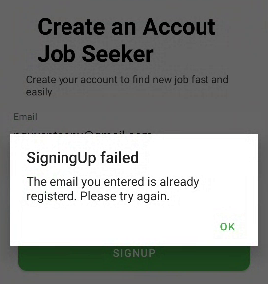
\includegraphics[width=.47\textwidth]{signin/fail}
        \noindent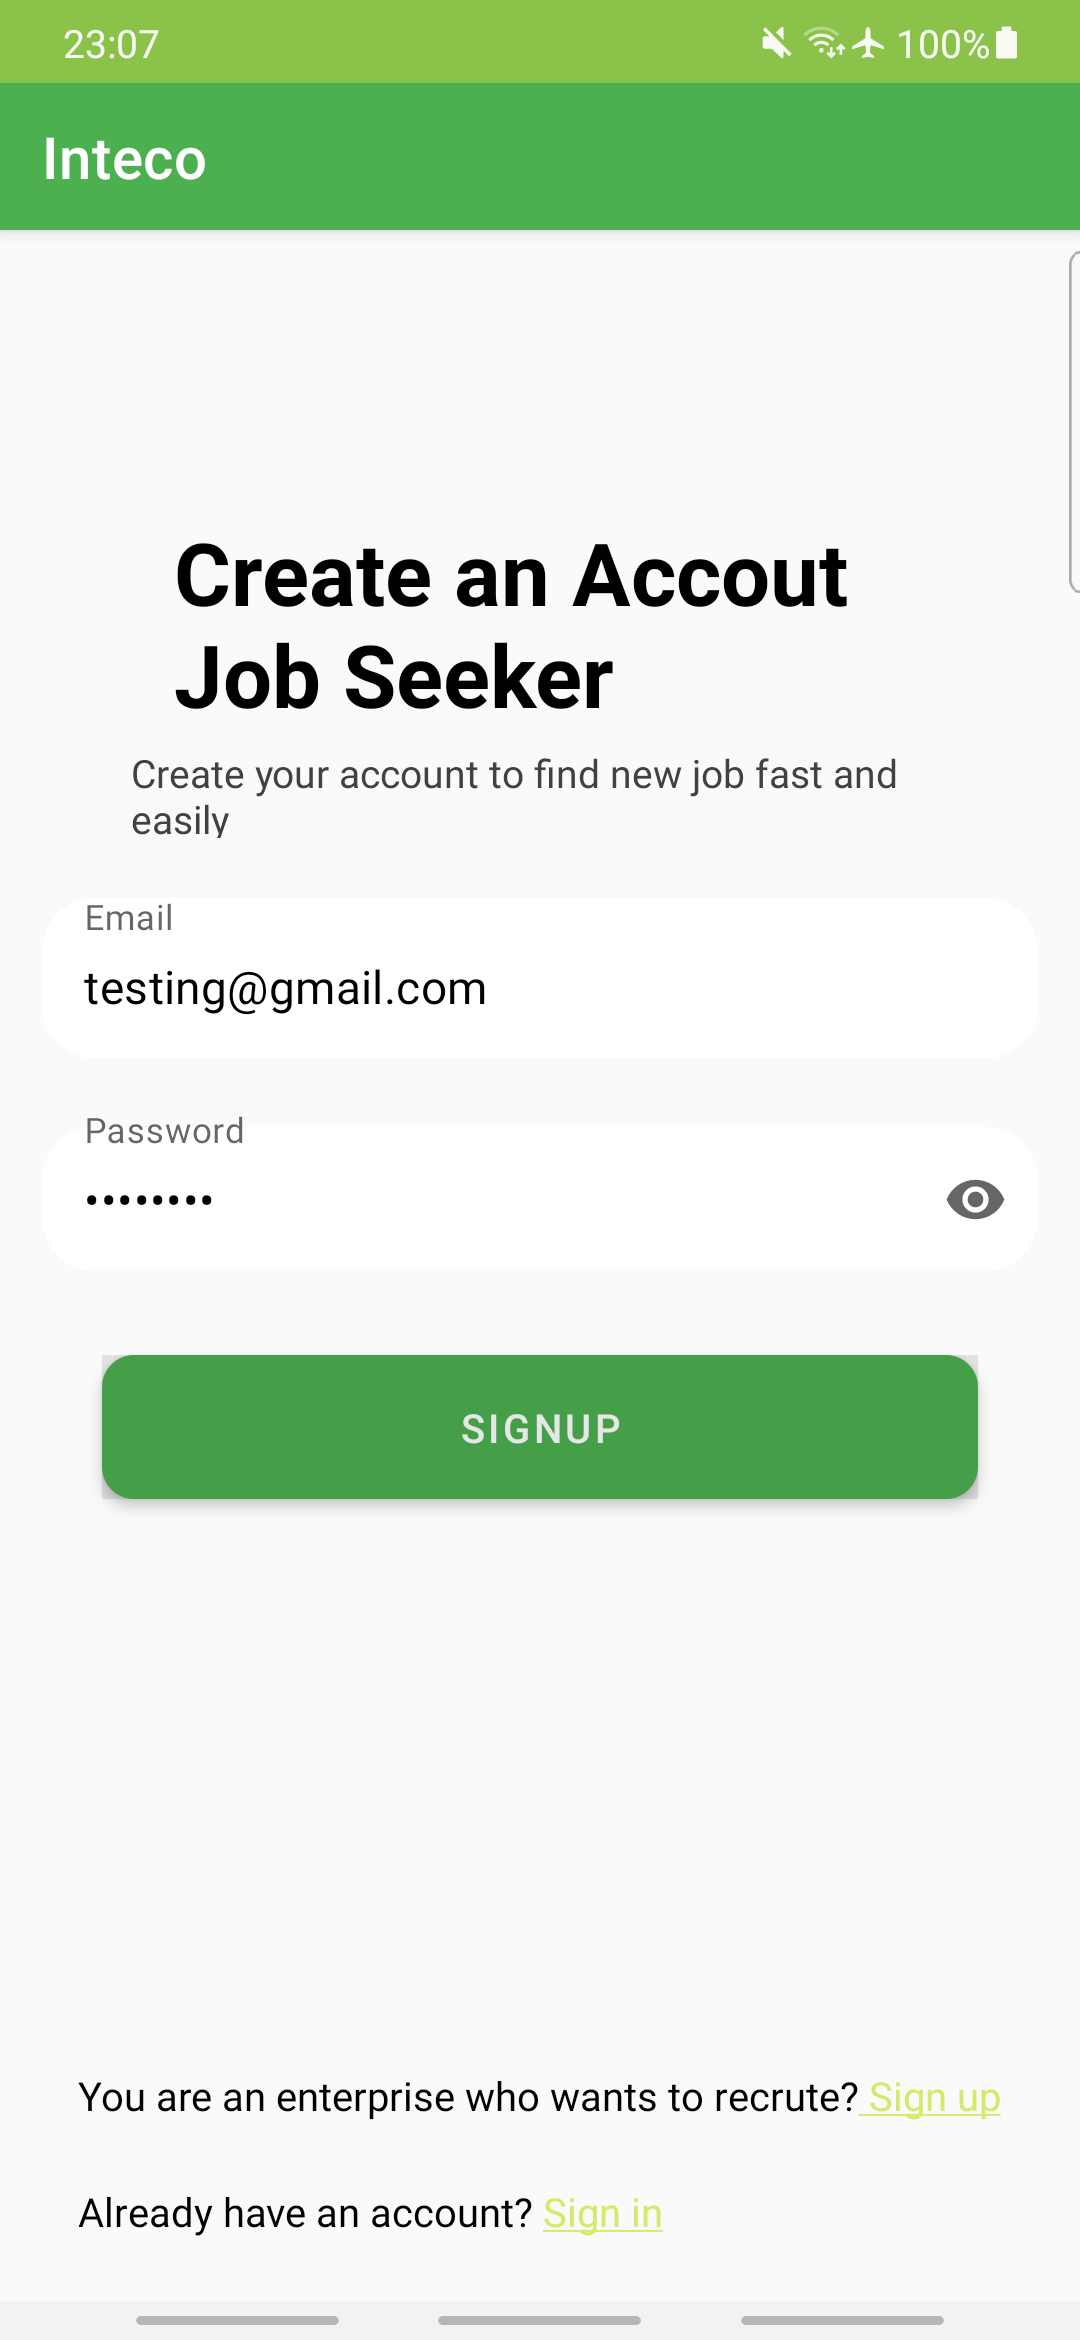
\includegraphics[width=.47\textwidth]{signin/page1}
        \noindent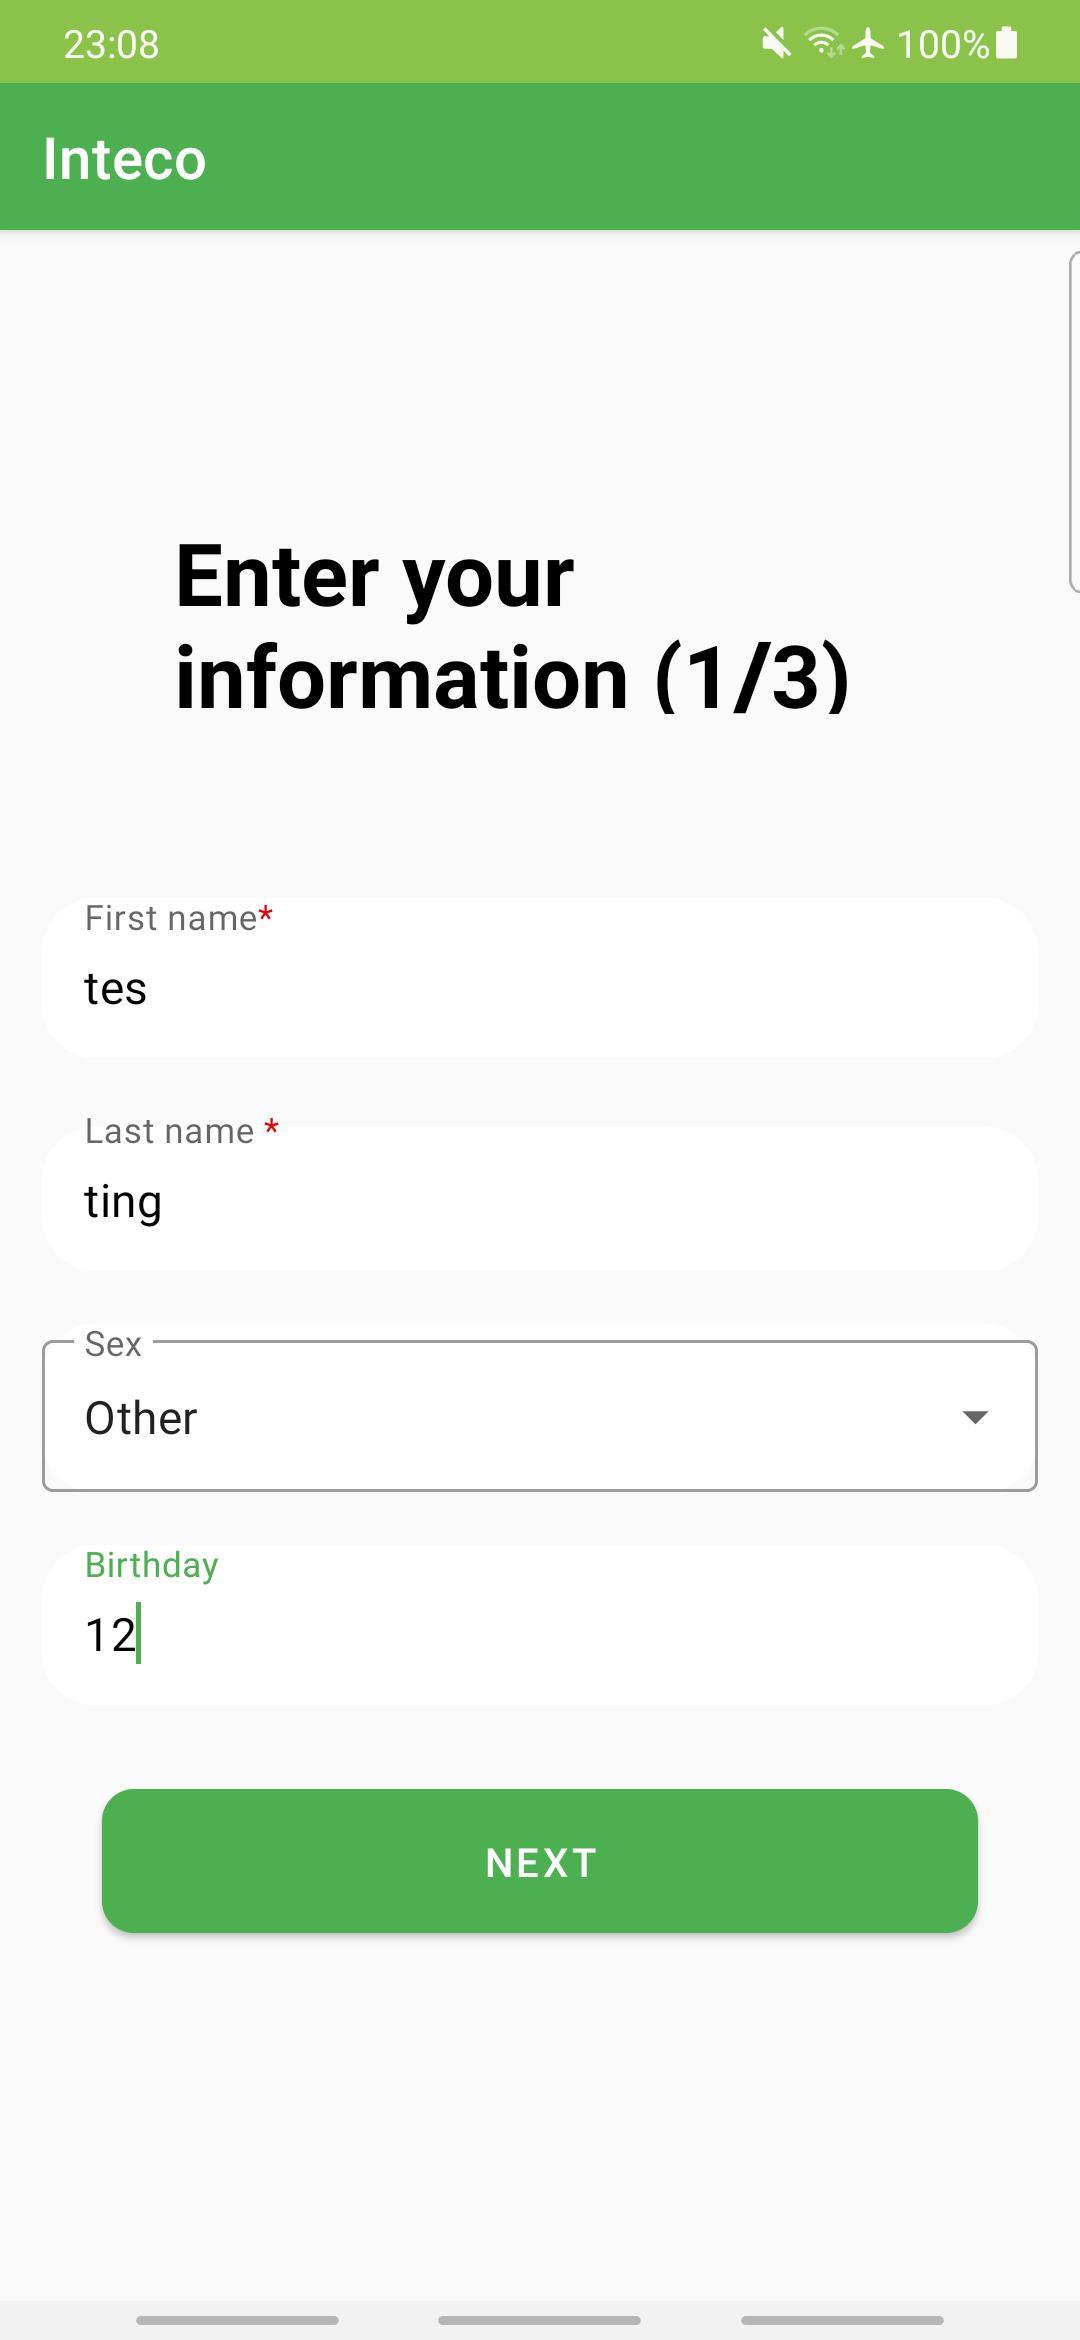
\includegraphics[width=.47\textwidth]{signin/page2}
        \noindent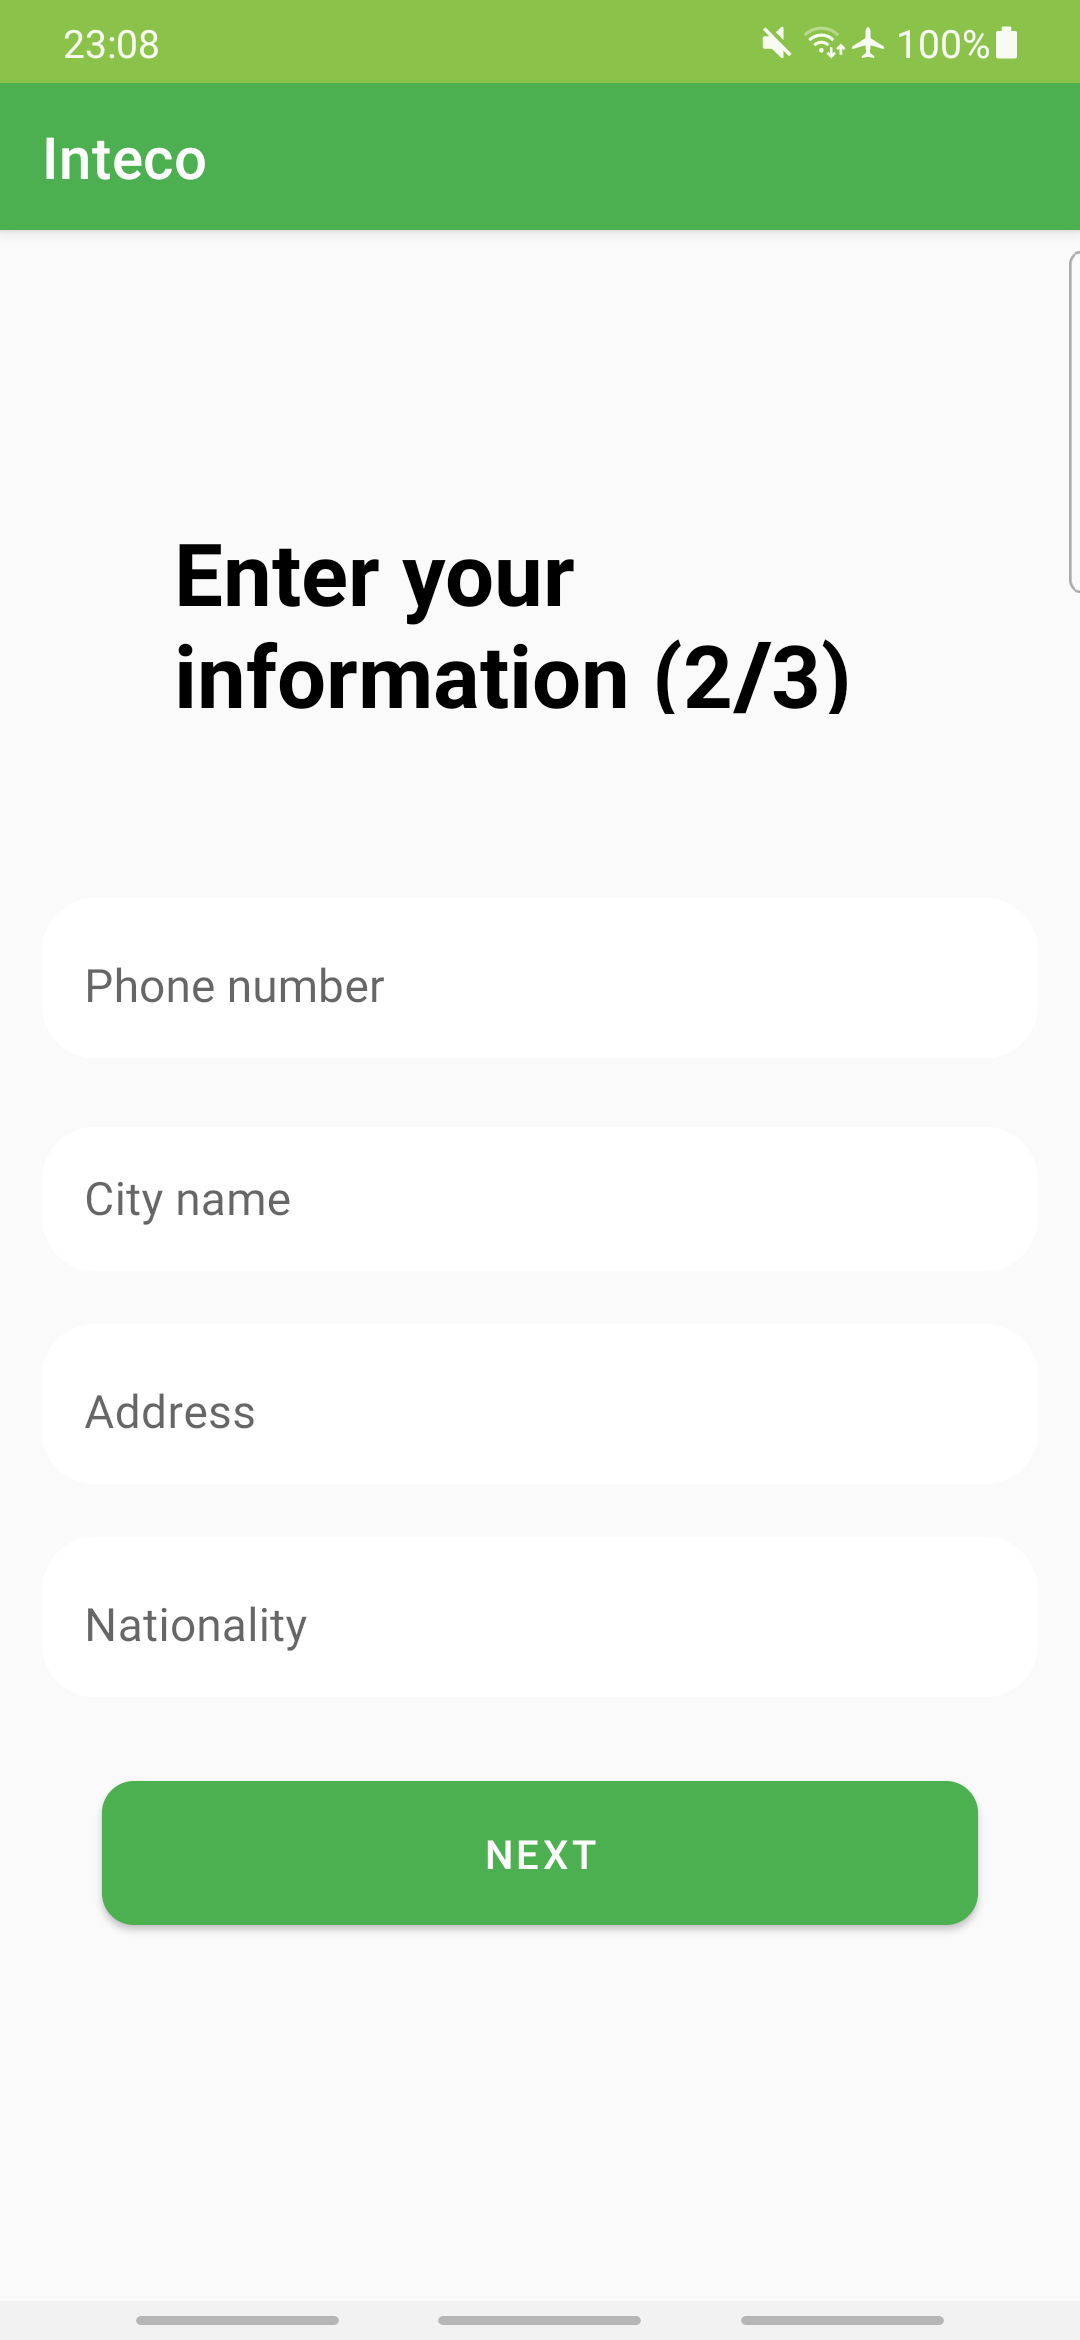
\includegraphics[width=.47\textwidth]{signin/page3}
        \noindent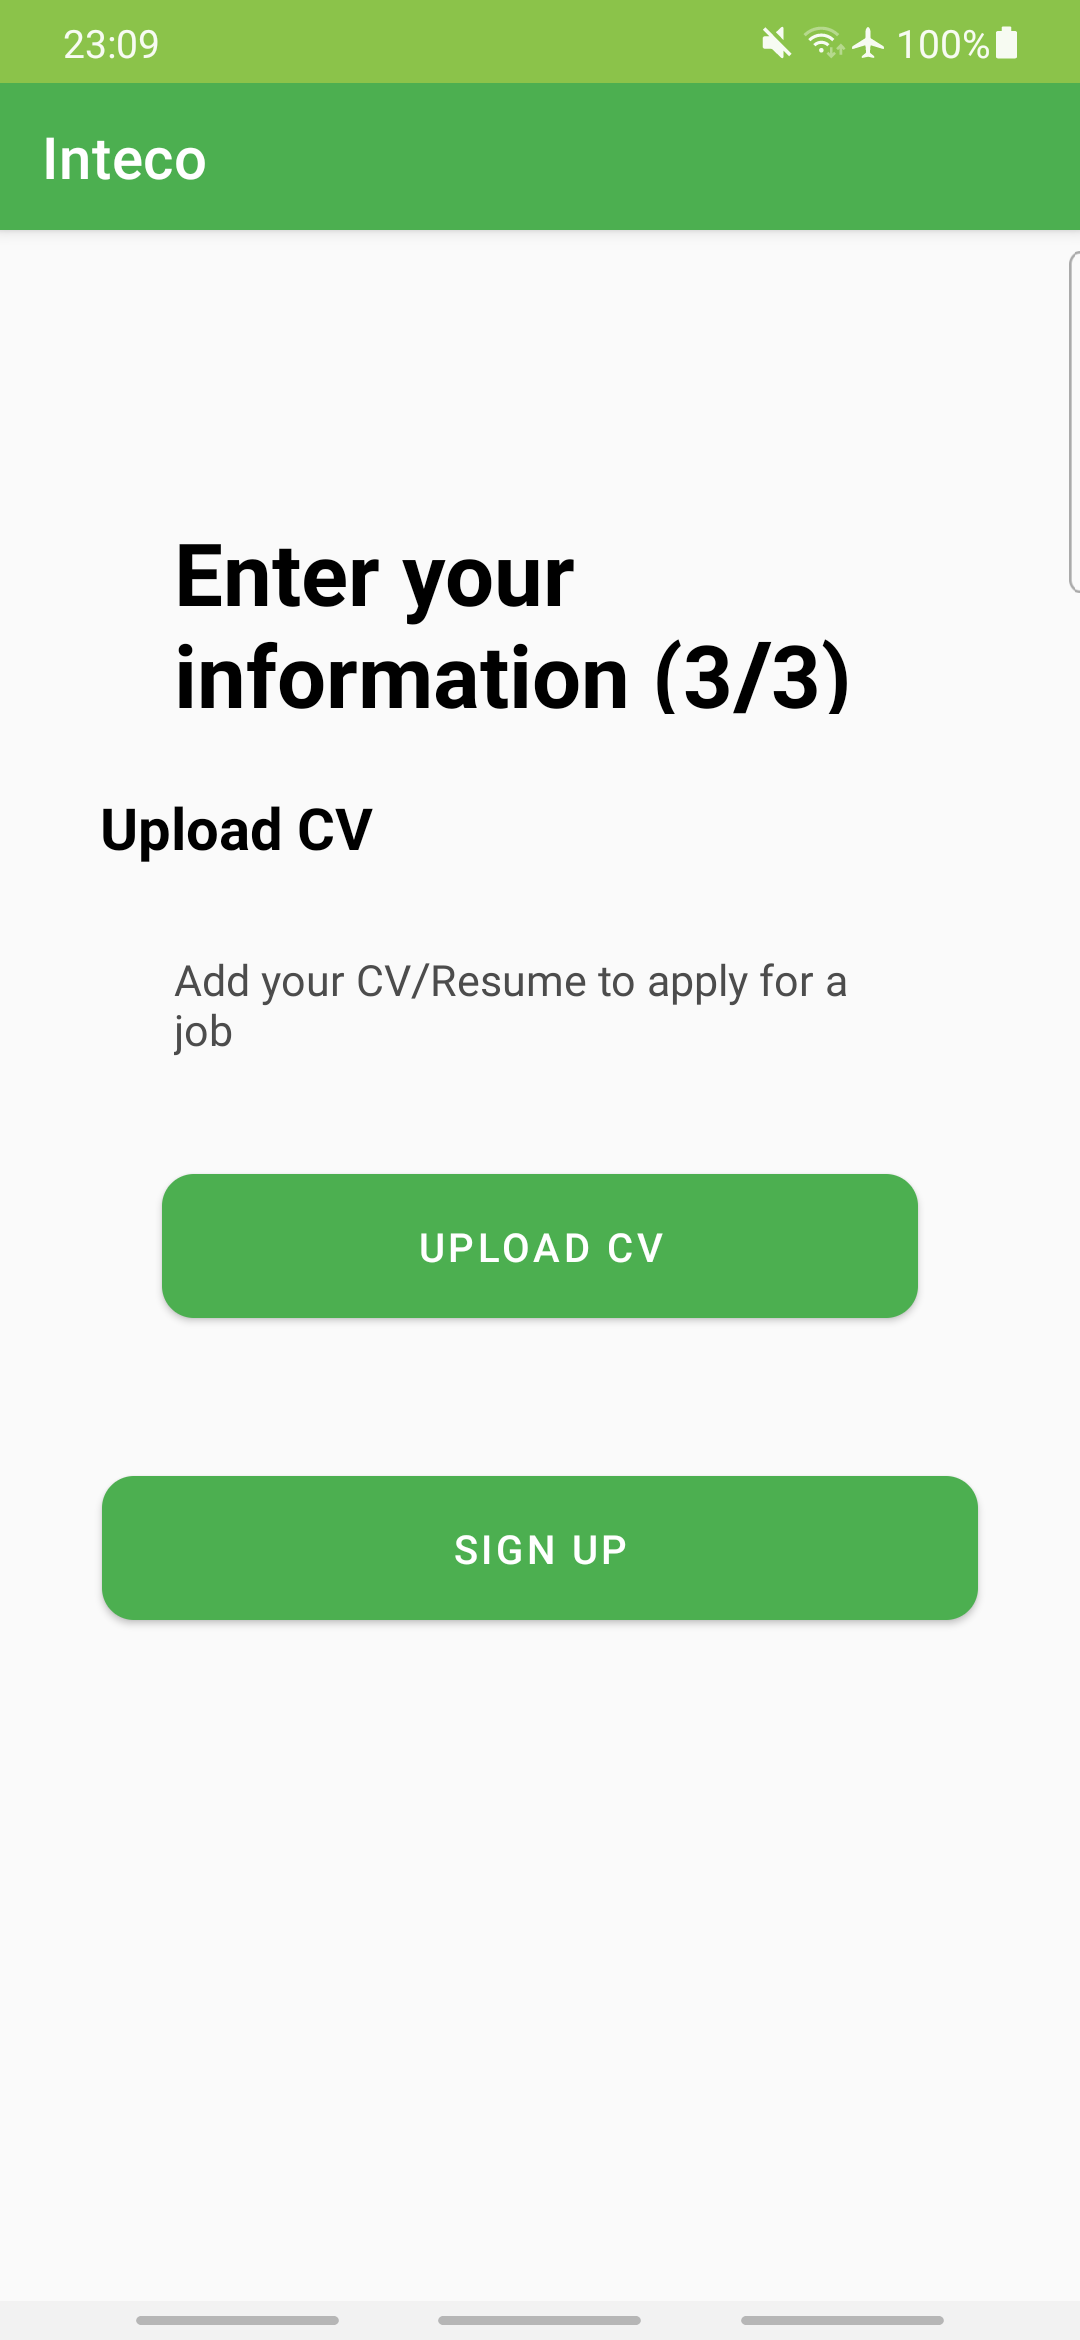
\includegraphics[width=.47\textwidth]{signin/page4}
        \noindent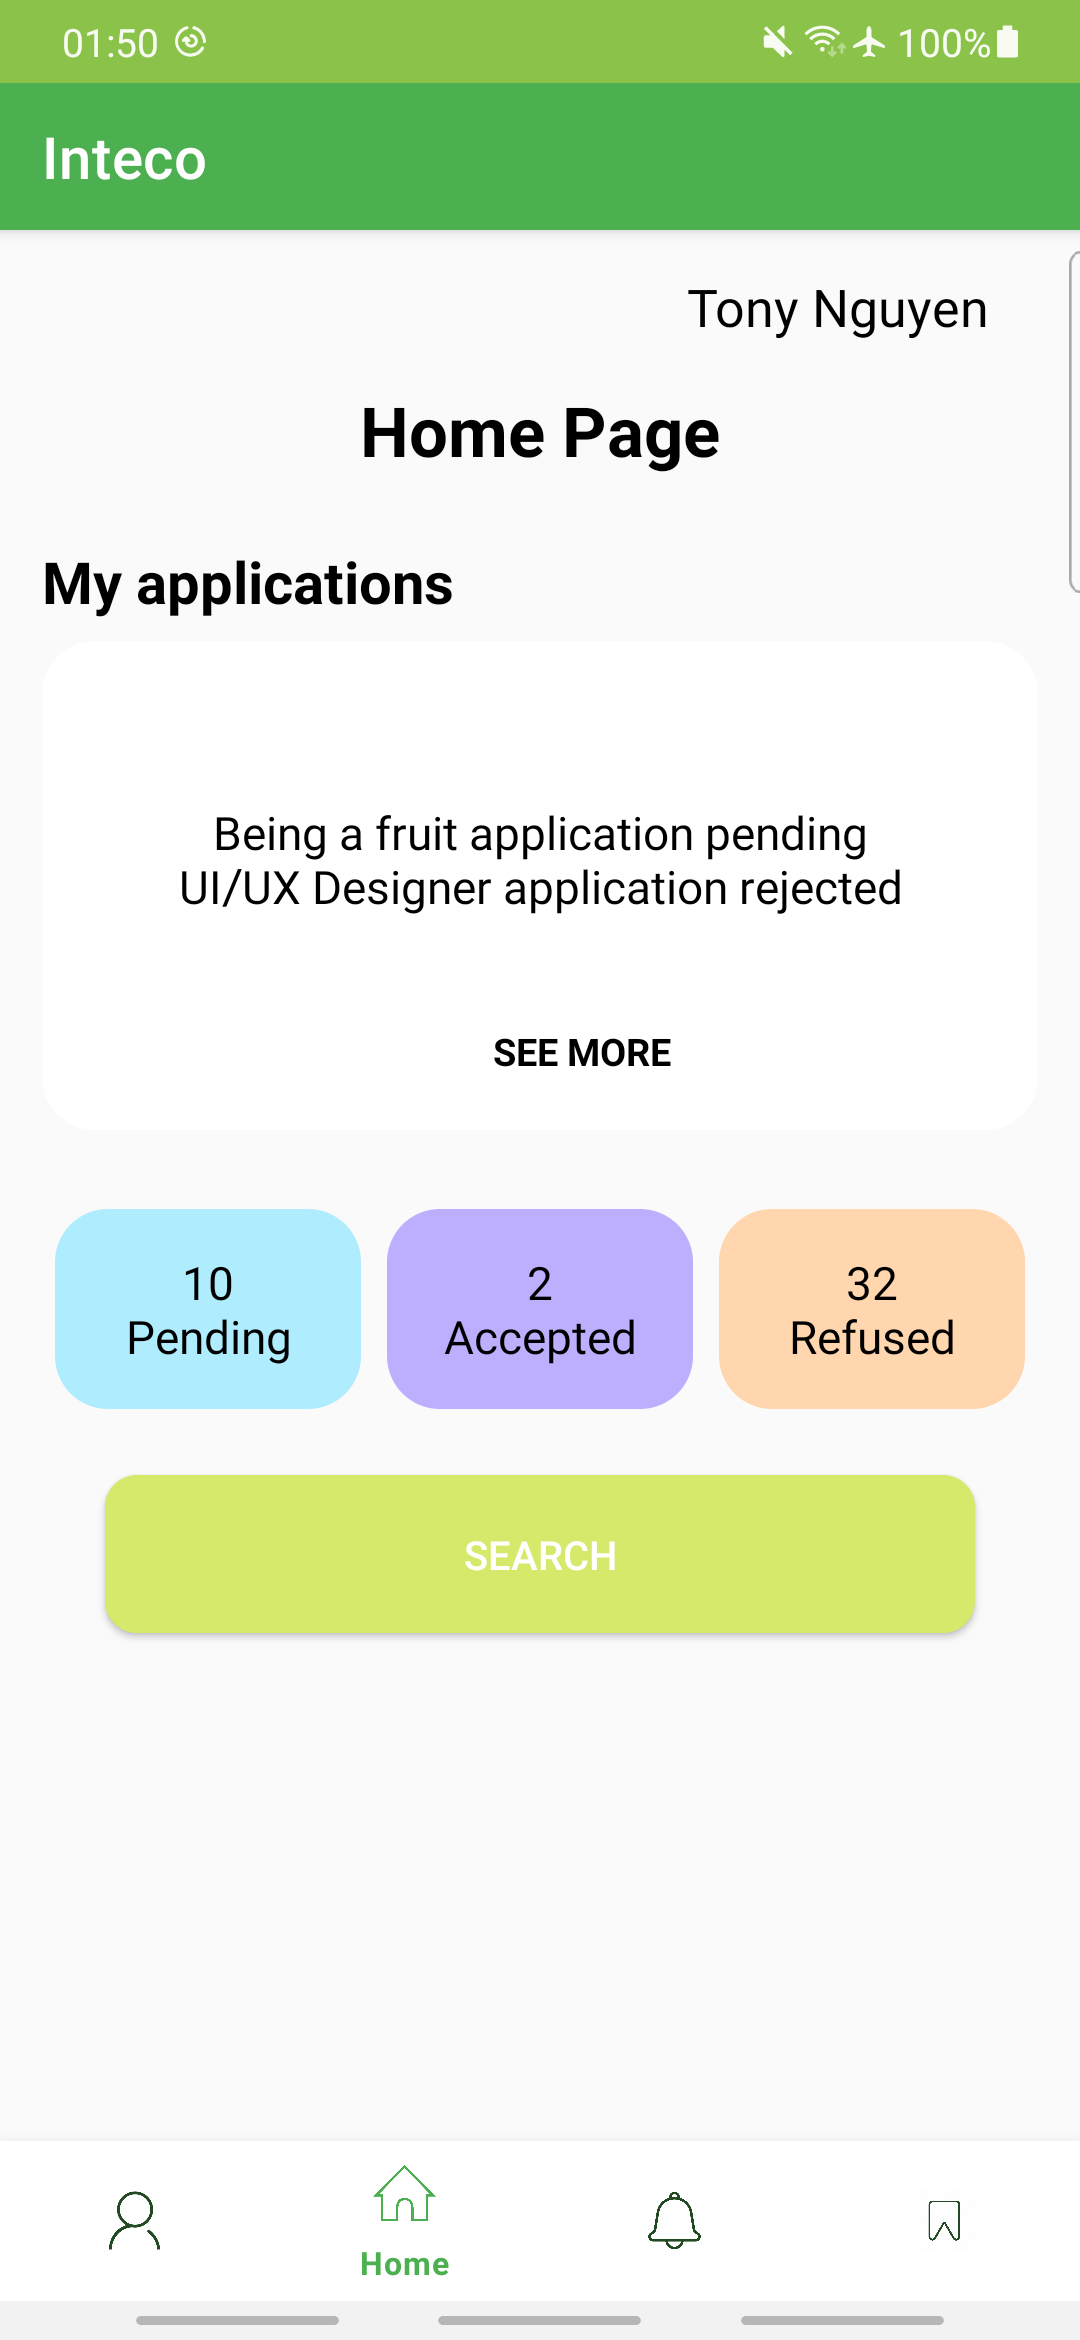
\includegraphics[width=.47\textwidth]{signin/after}
        \noindent\includegraphics[width=.47\textwidth]{signin/code}
        \subsection{La connection}
        \paragraph{}
        Les utilisateurs peuvent se connecter du même endroit, qu'ils soient entreprise ou chomeurs.
        
        \noindent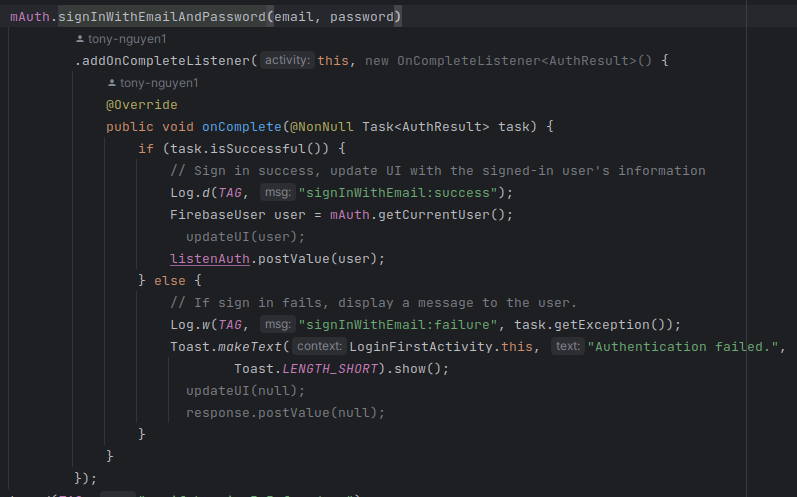
\includegraphics[width=.47\textwidth]{login/signInWithEmailAndPassword}
        \subsection{Changement de mot de passe}
        \paragraph{}
        Les utilisateurs peuvent changer leur mot de passe. En effet, ils ont la possibilité de recevoir un mail pour faire ça grace au service Authentification de Firebase.

        \noindent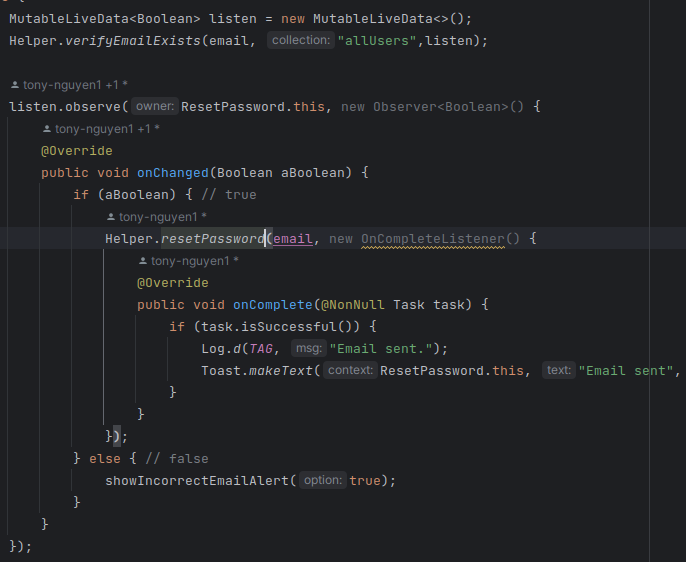
\includegraphics[width=.47\textwidth]{resetPwd/codeReset}
        \noindent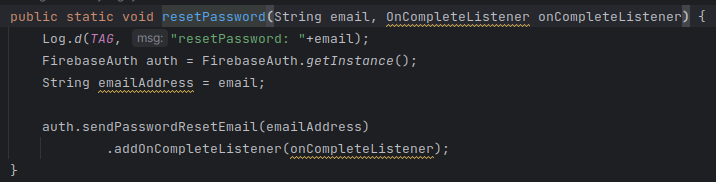
\includegraphics[width=.47\textwidth]{resetPwd/codeResetAuth}
        \noindent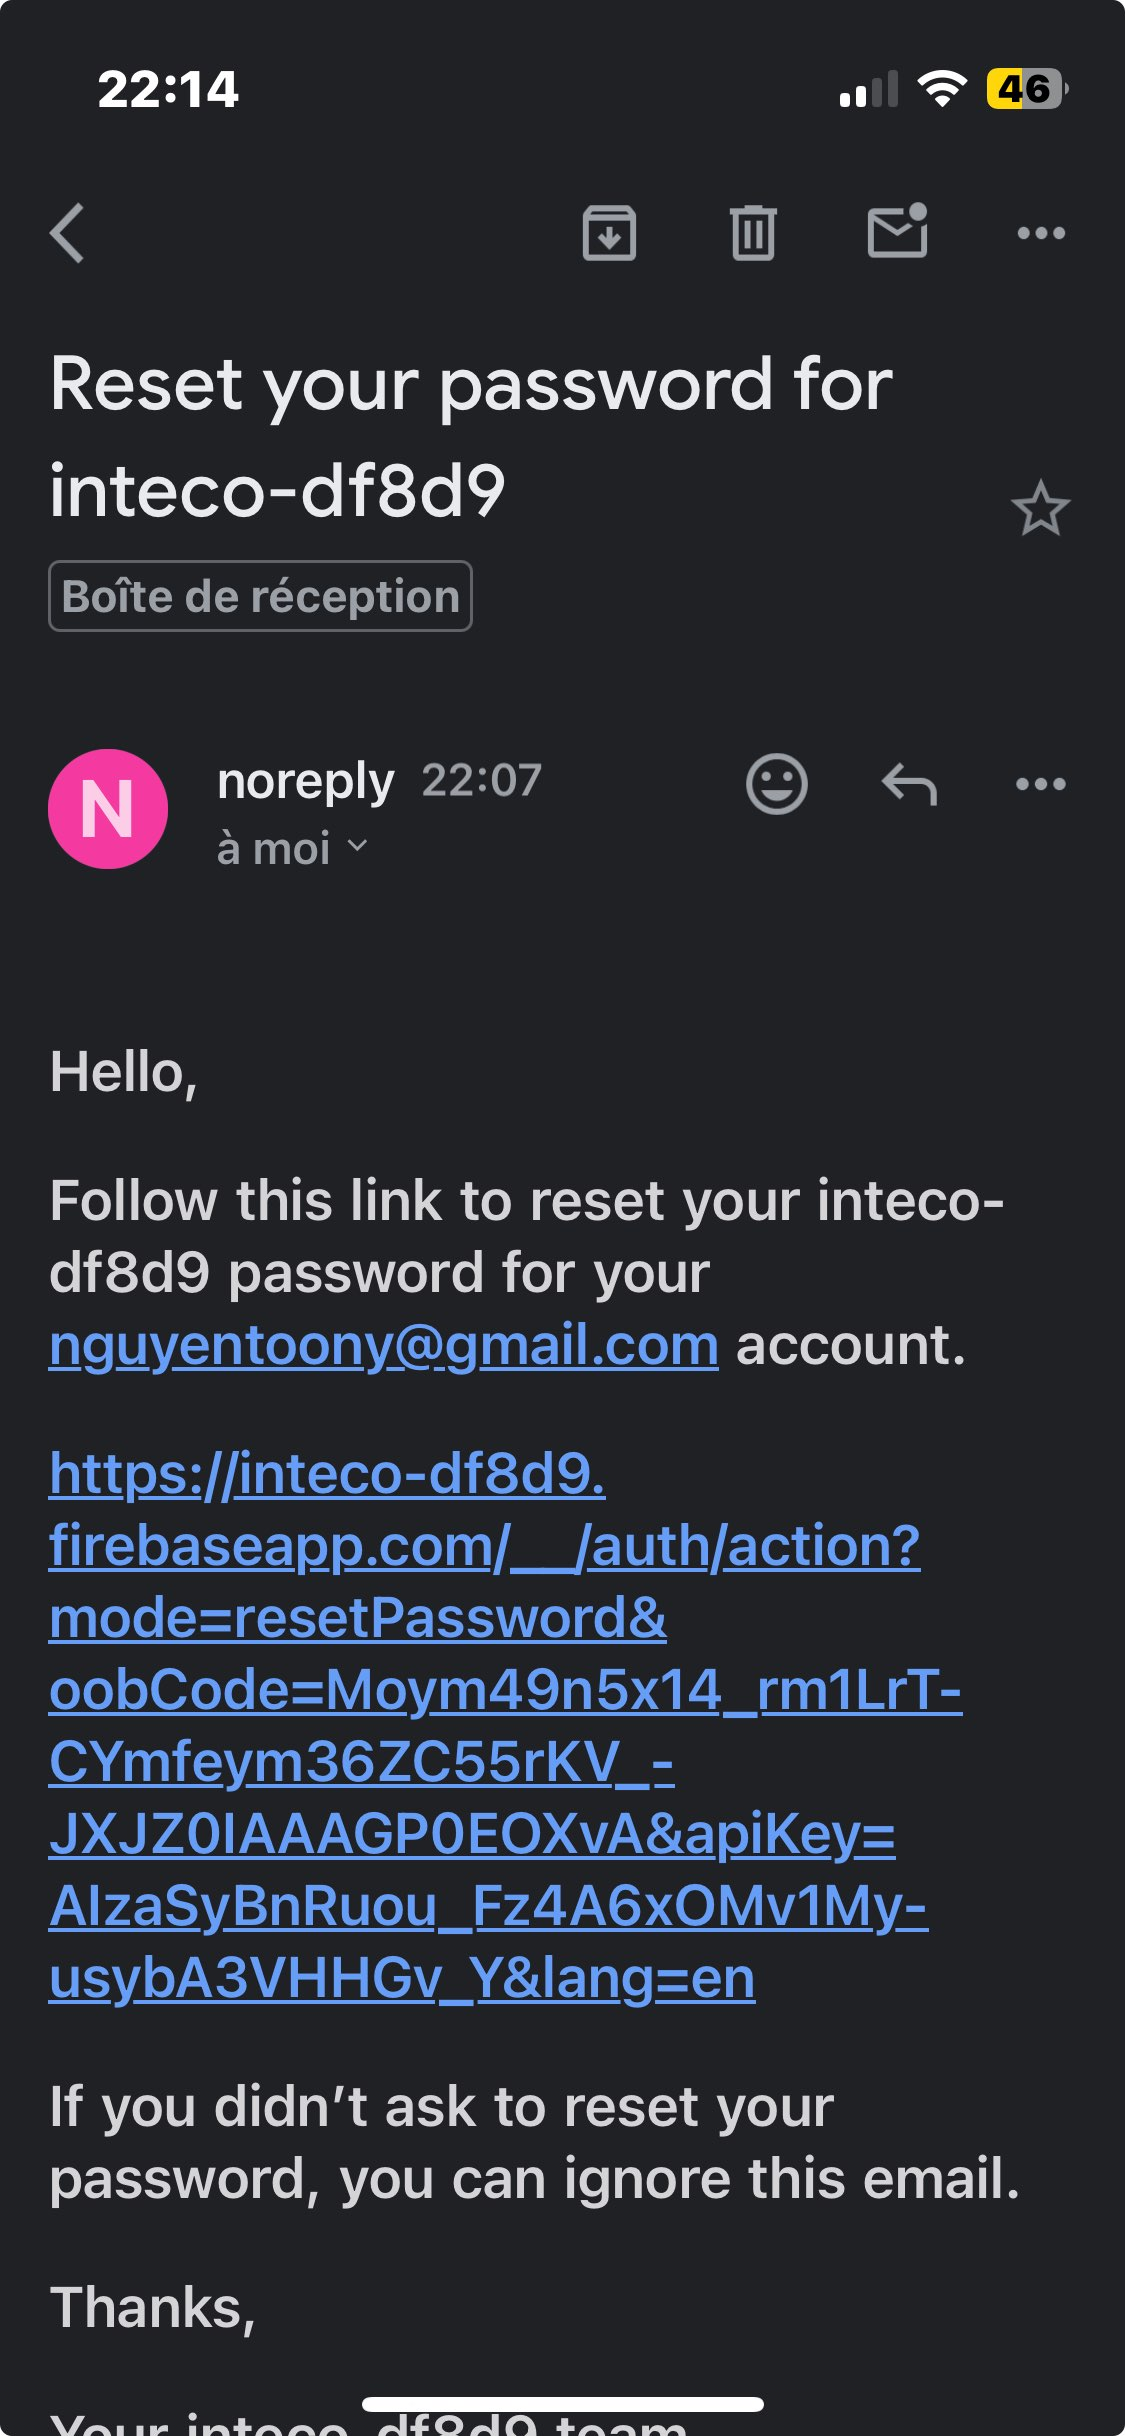
\includegraphics[width=.47\textwidth]{resetPwd/result}
        \subsection{Barre de navigation}
        La page principale après la connection est une activité. La navigation vous fait passer d'un fragment à l'autre.

        \noindent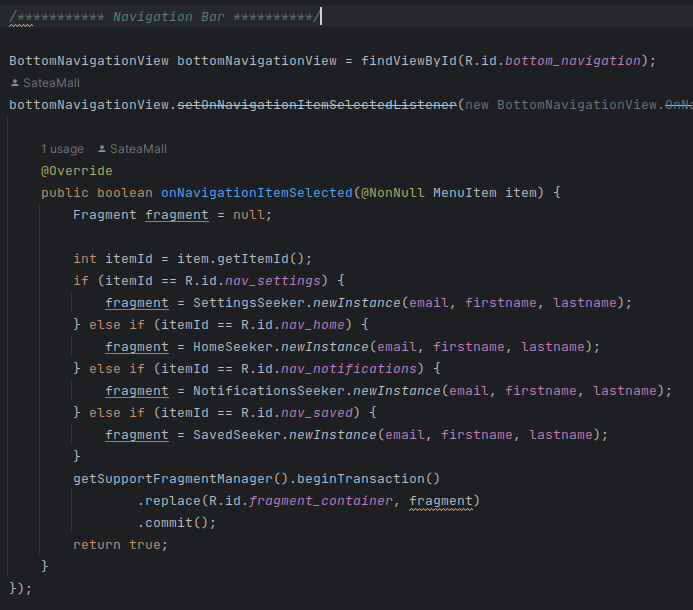
\includegraphics[width=.47\textwidth]{navBar/codeNavBar}
        \noindent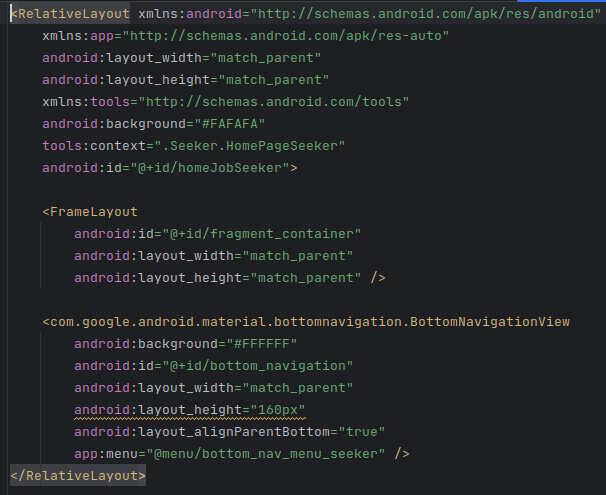
\includegraphics[width=.47\textwidth]{navBar/layoutNavBar}
        \subsection{Sauvegarder}
        \paragraph{}
        Si jamais, un chercheur de travail souhaite revenir à une offre d'emplois, il a la possibilité de l'enregistrer.

        \noindent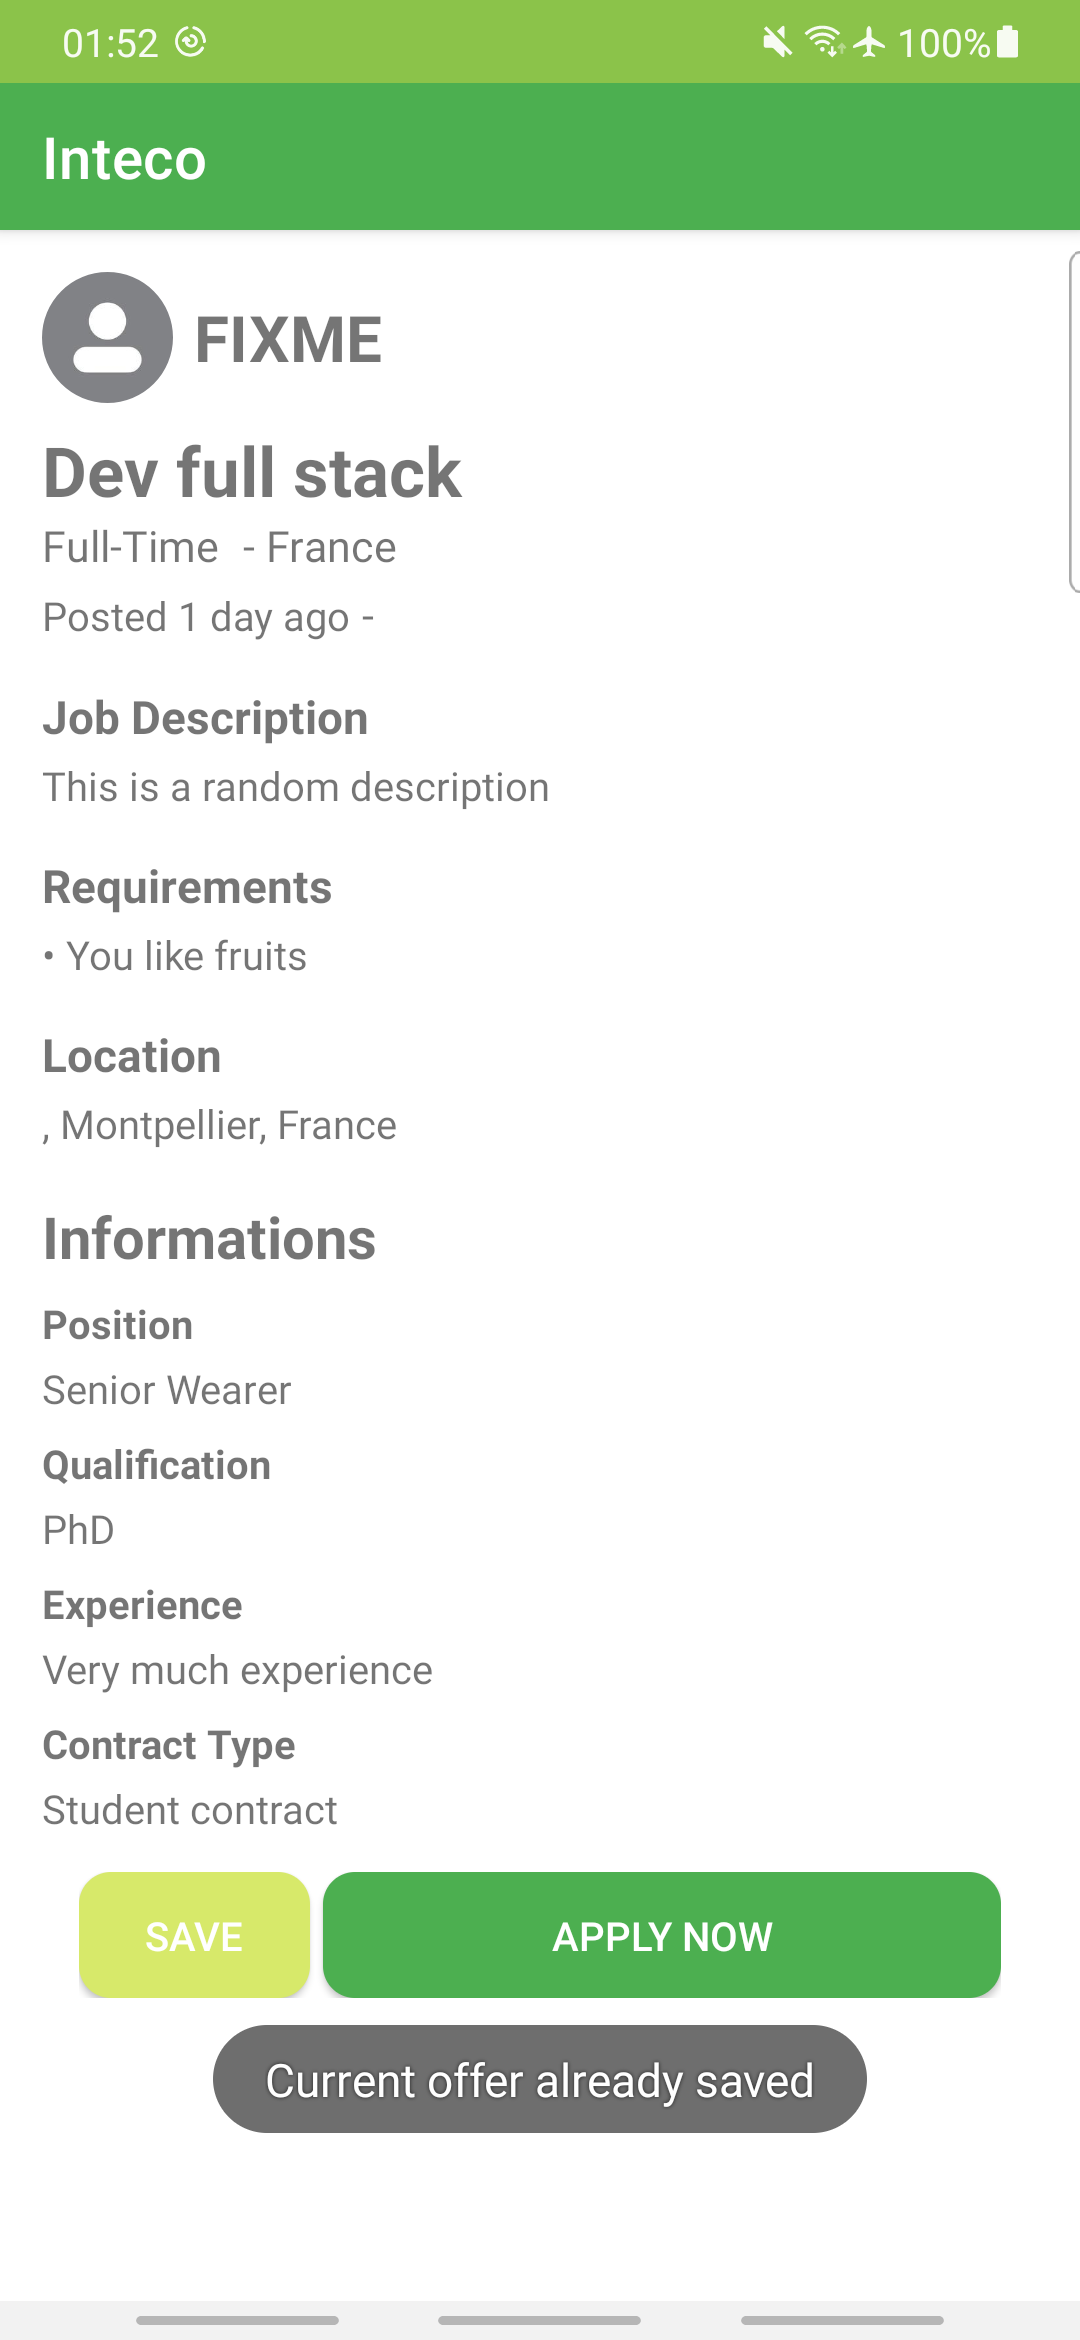
\includegraphics[width=.47\textwidth]{save/screenSave}
        \noindent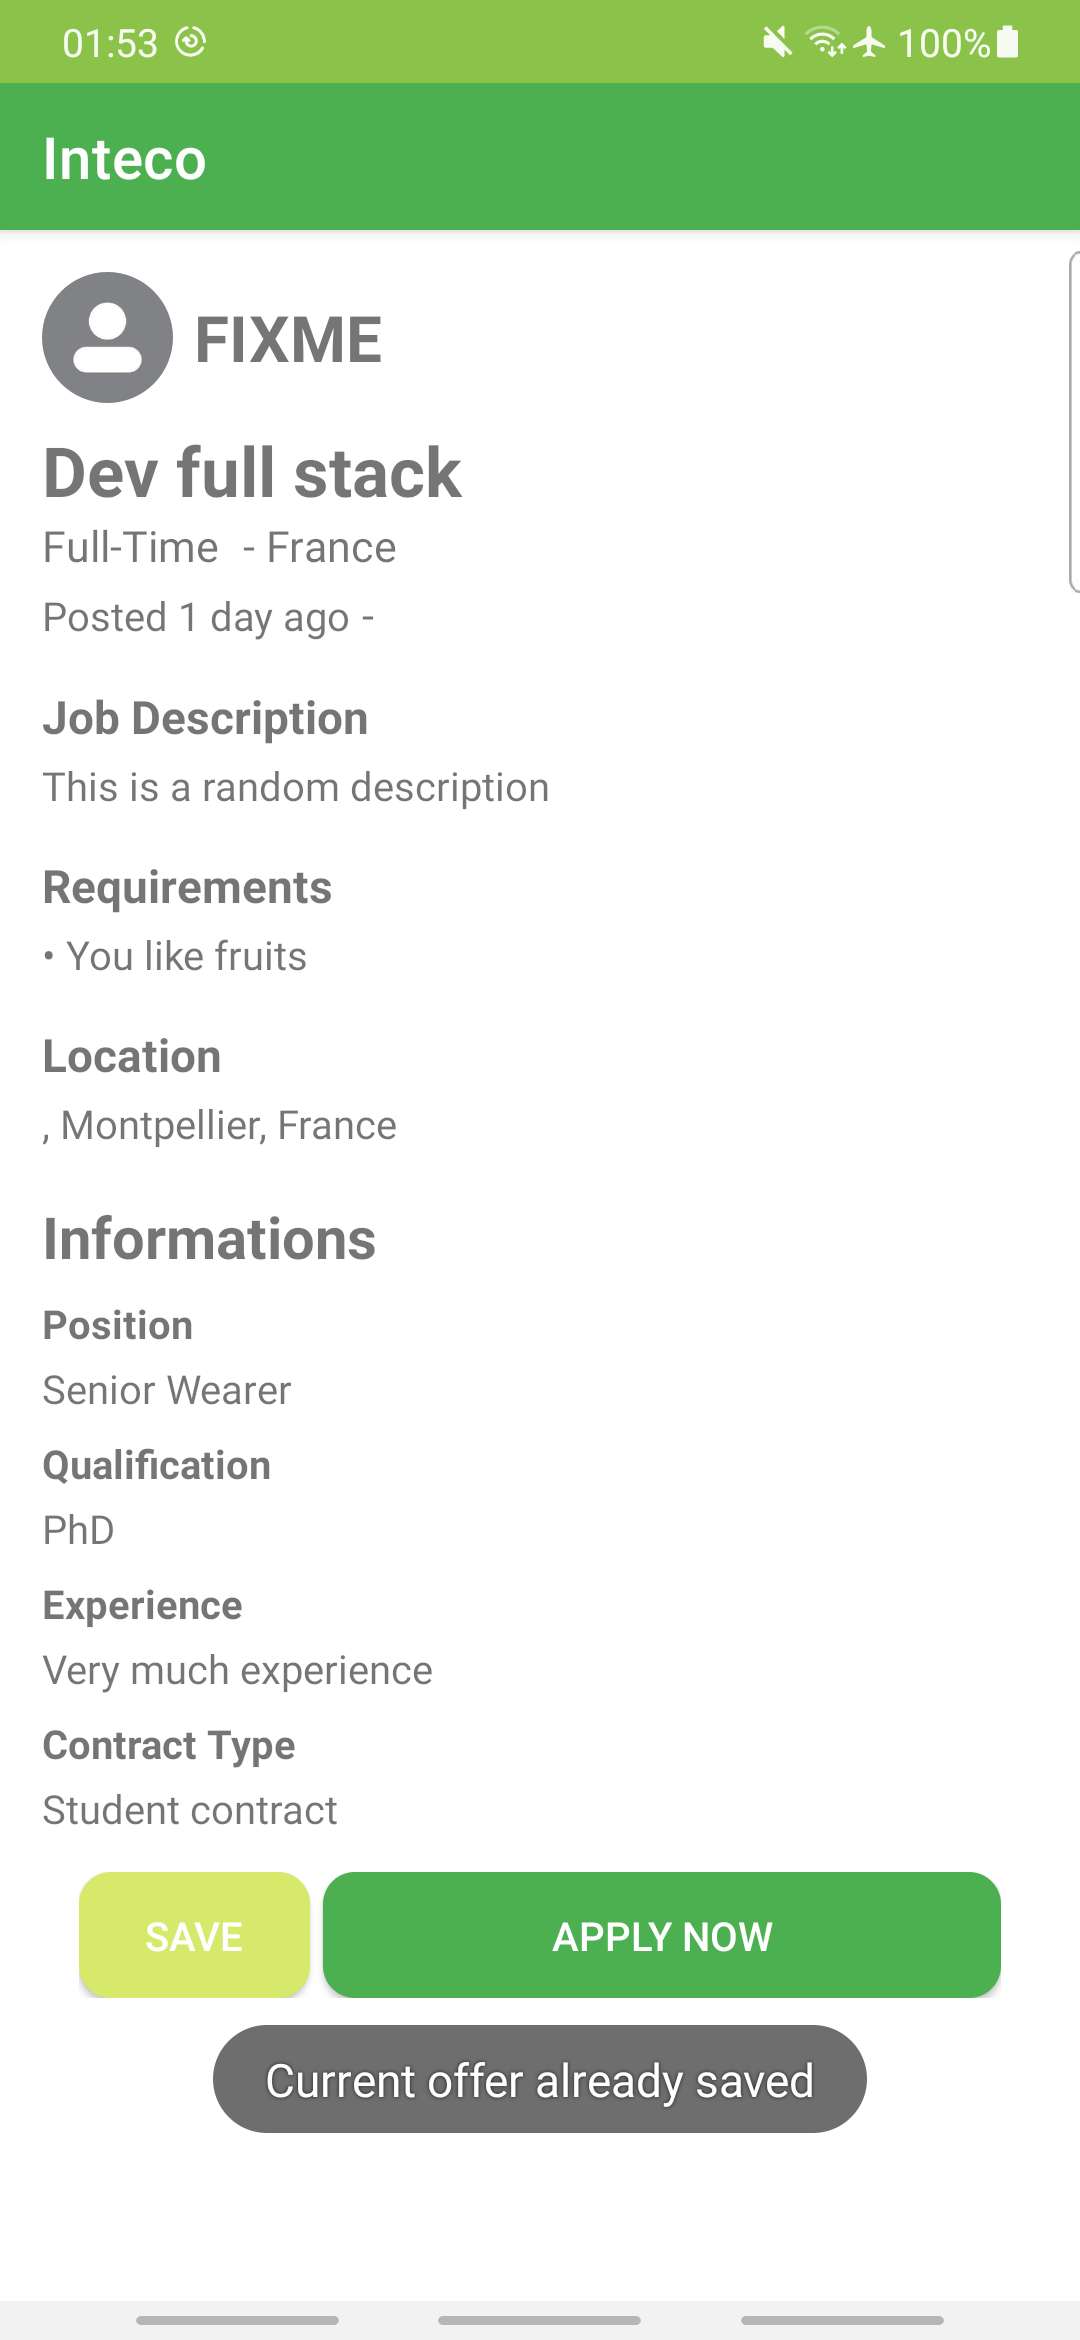
\includegraphics[width=.47\textwidth]{save/alreadySaved}
        \noindent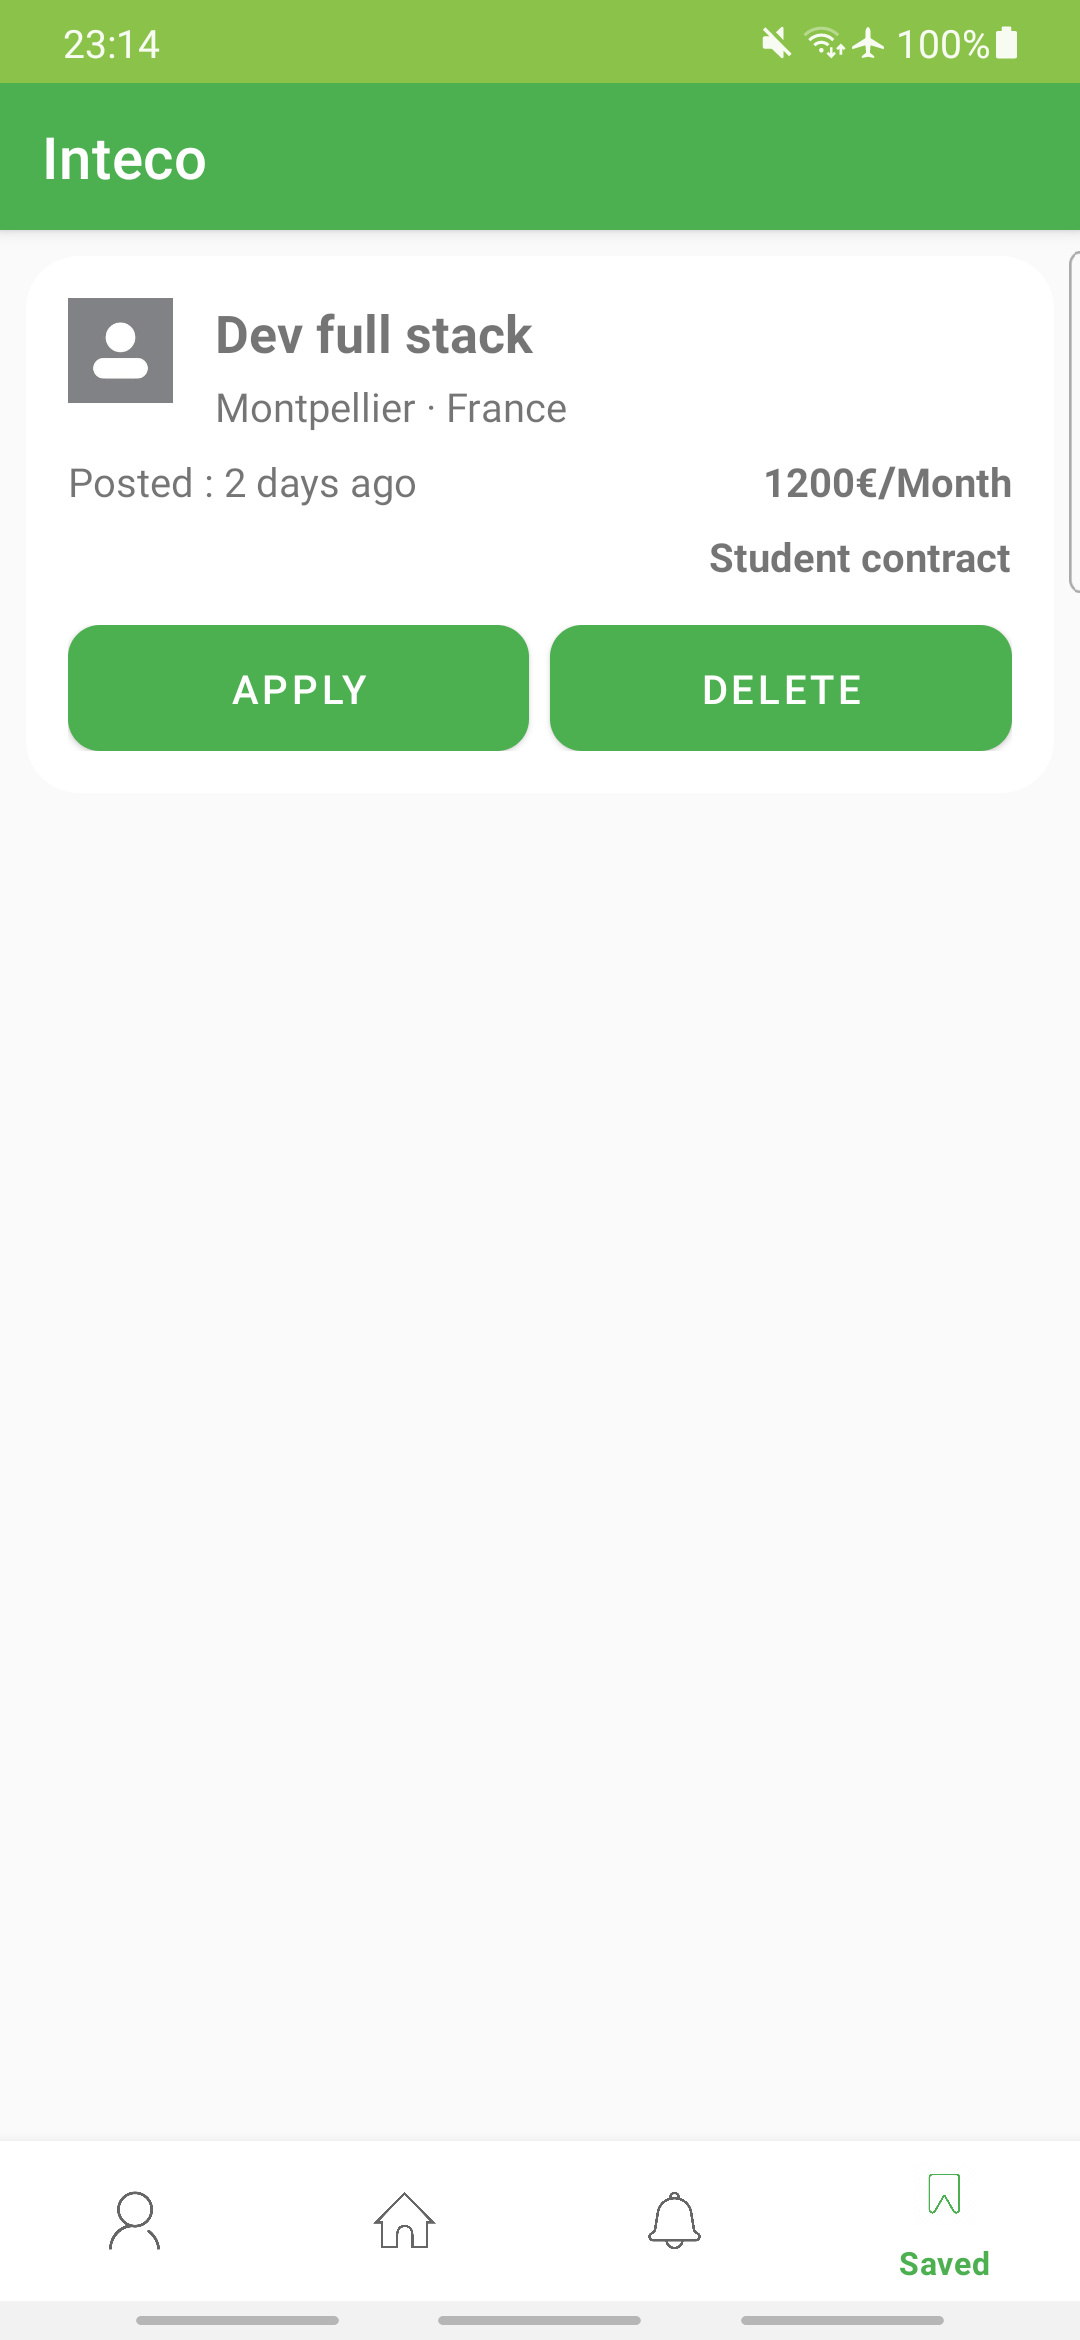
\includegraphics[width=.47\textwidth]{save/screenSavedList}
        \noindent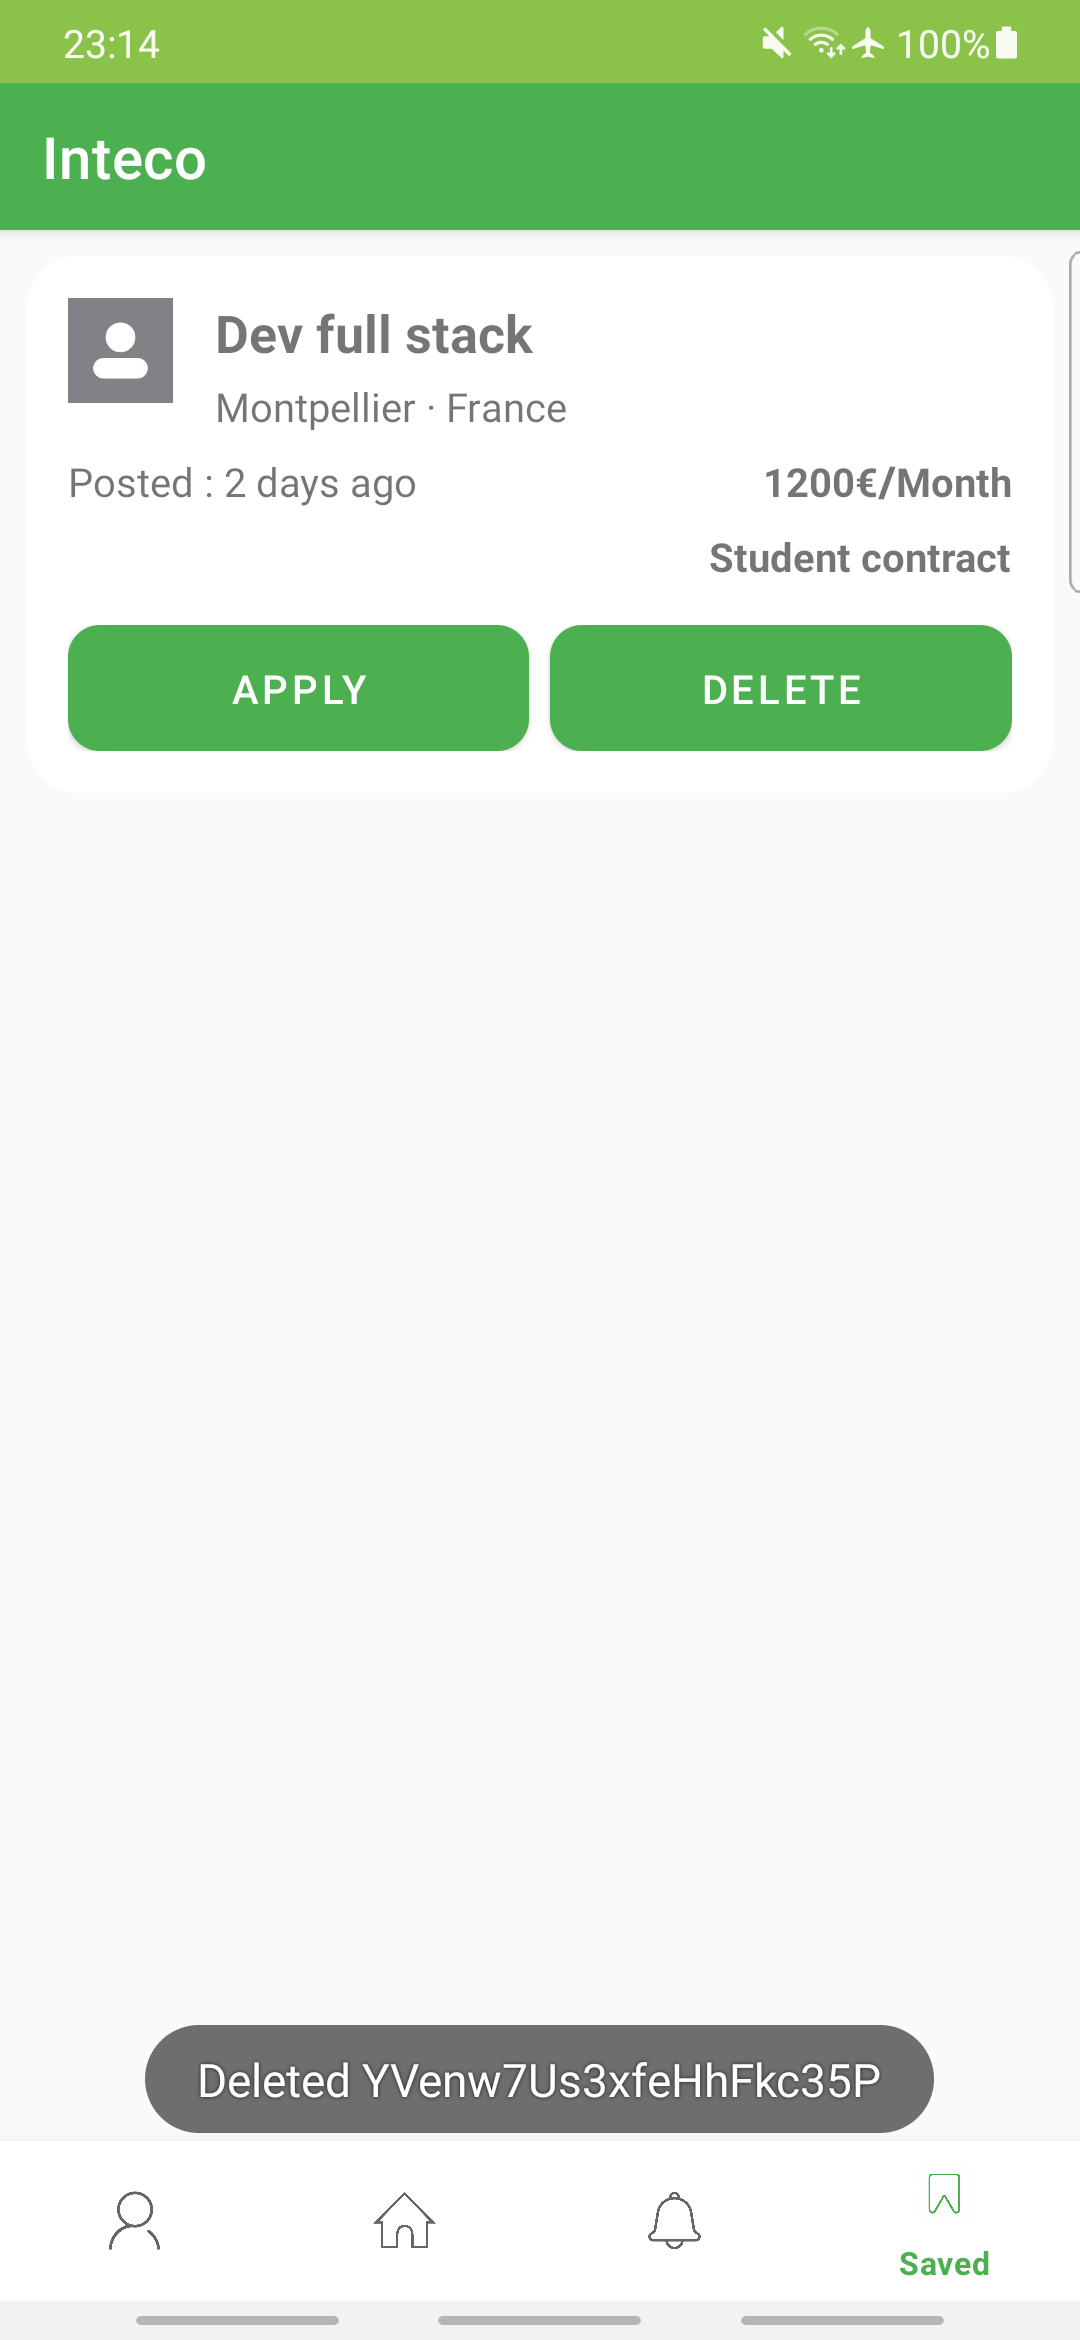
\includegraphics[width=.47\textwidth]{save/screenDelete}
        \noindent\includegraphics[width=.47\textwidth]{save/code}
        \subsection{Postuler}
        \paragraph{}
        Un chercheur d'emplois peut postuler a une offre.

        \noindent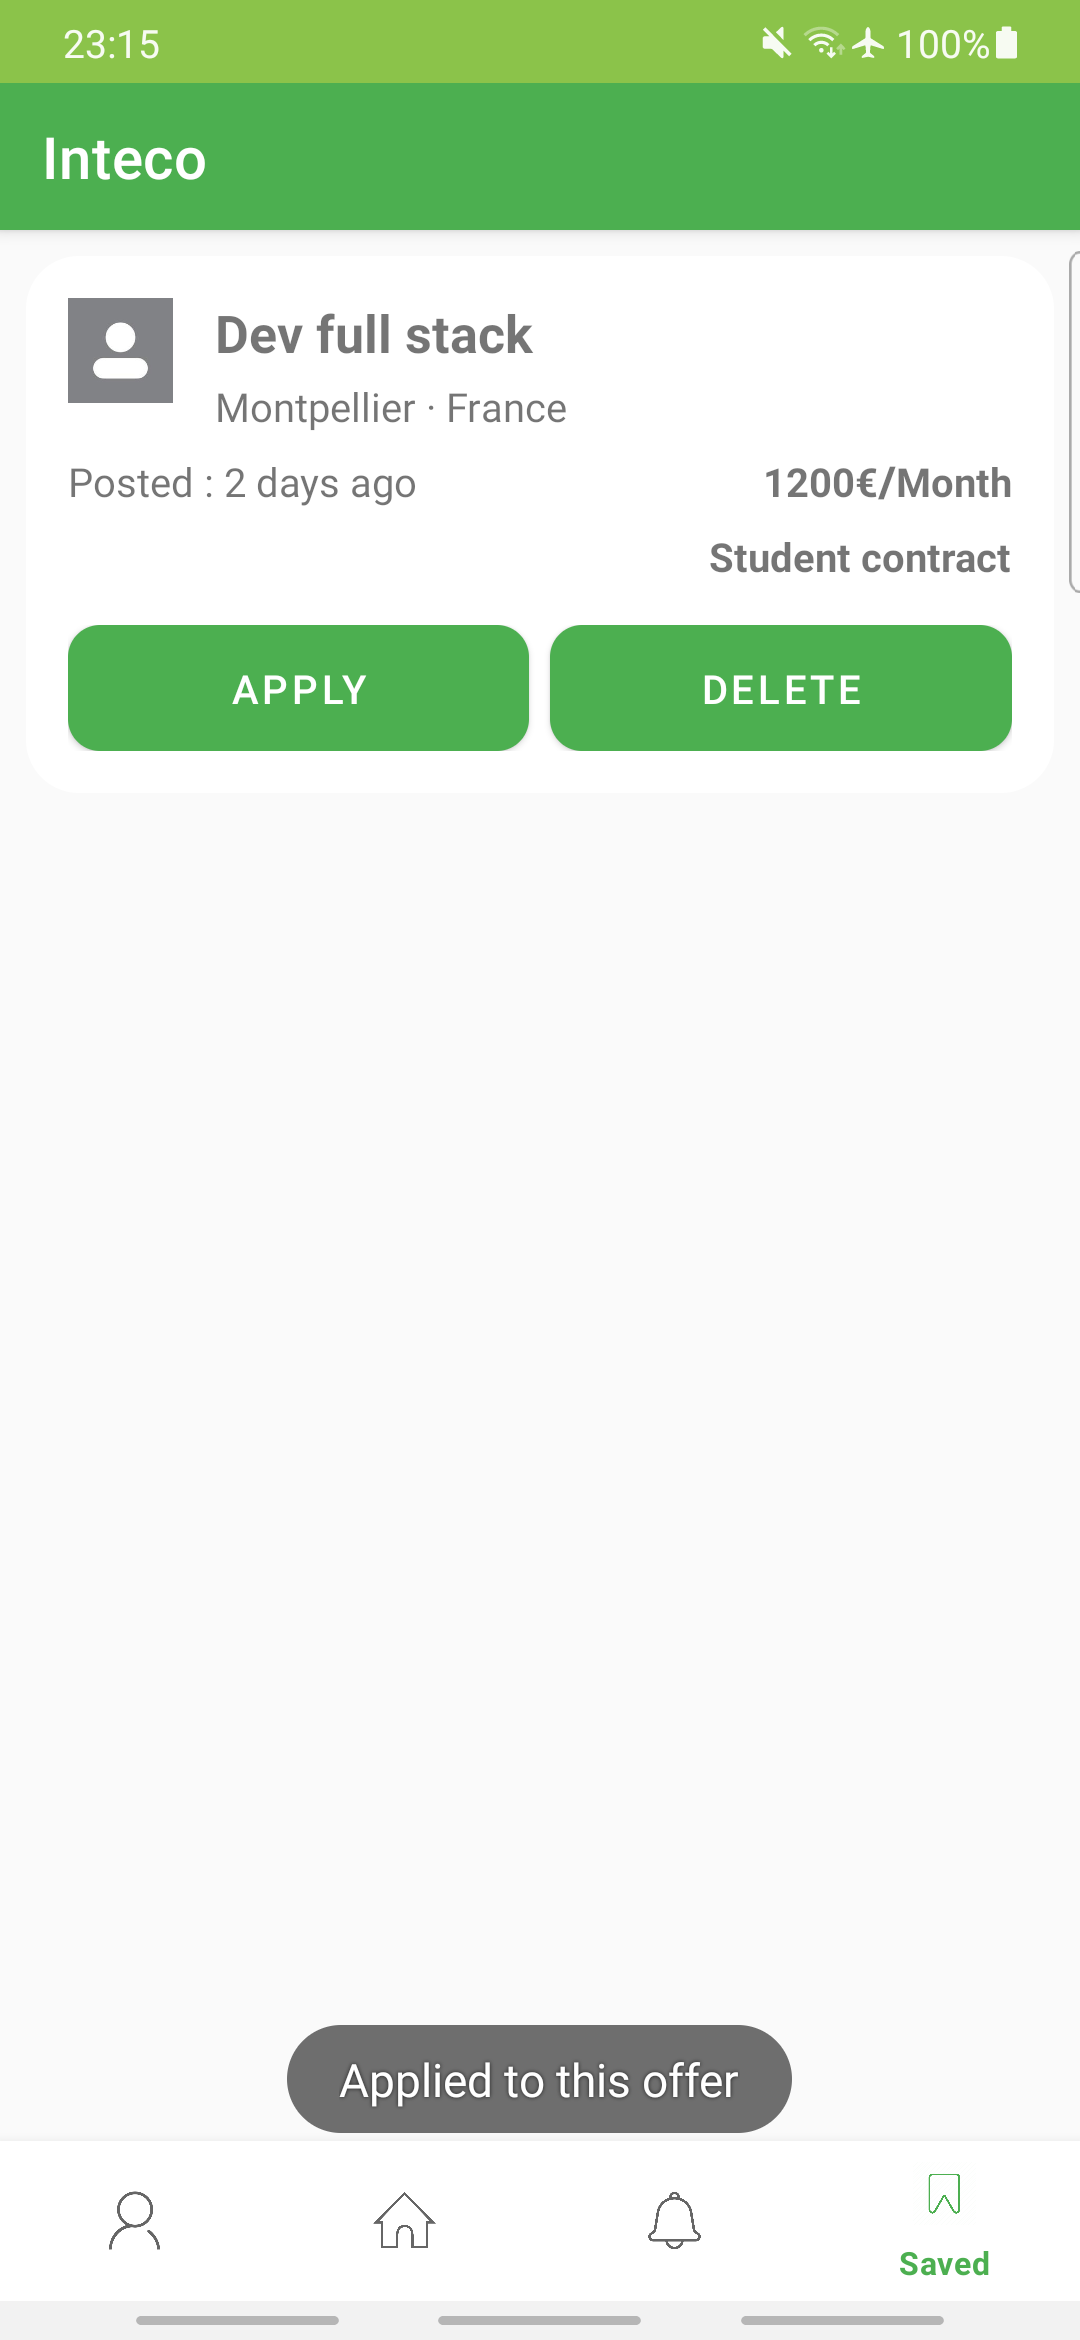
\includegraphics[width=.47\textwidth]{apply/screenApplied}
        \noindent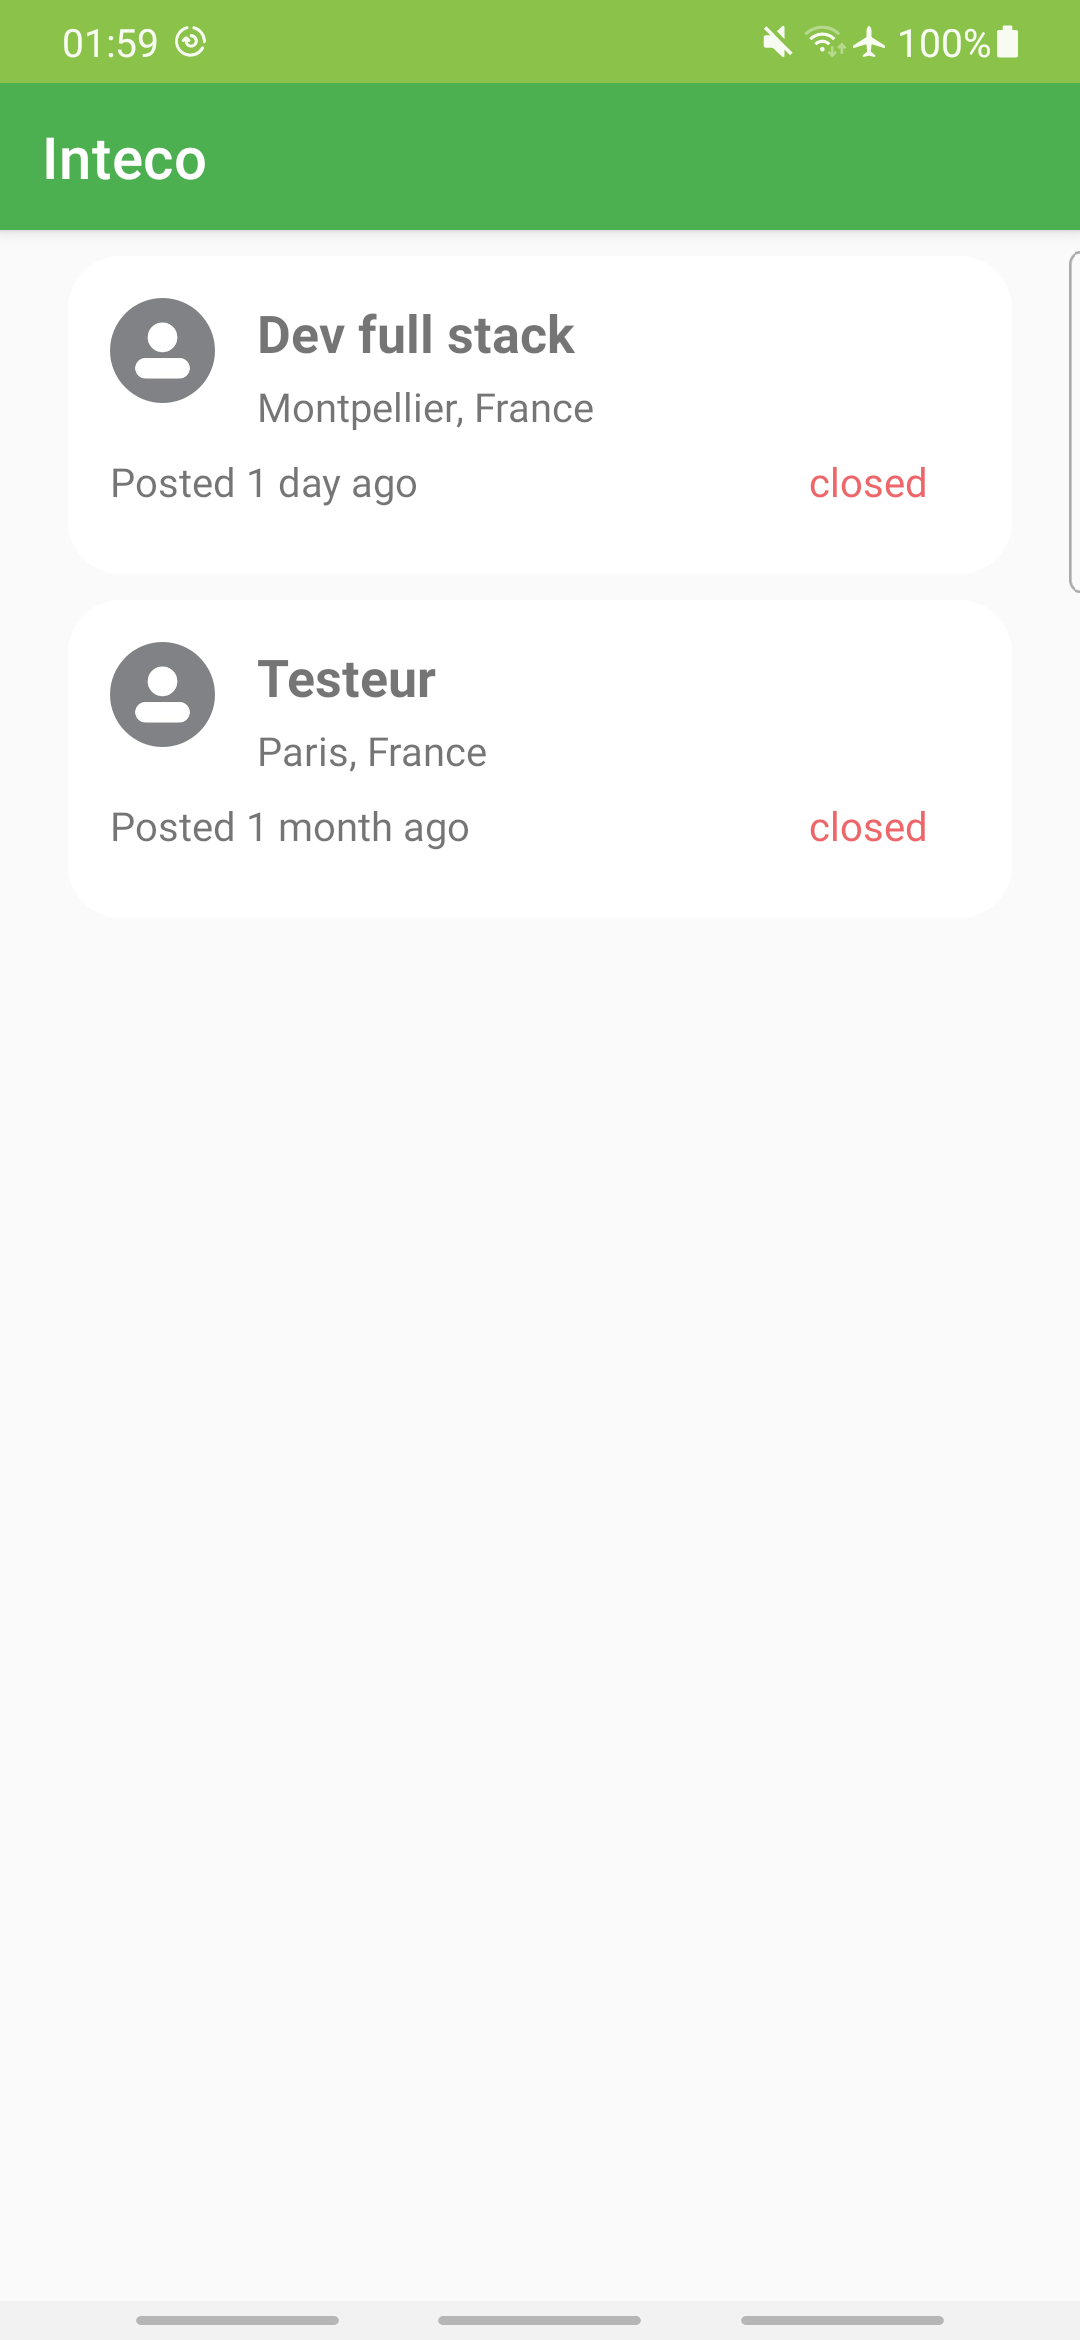
\includegraphics[width=.47\textwidth]{apply/screenAppliedList}
        \noindent\includegraphics[width=.47\textwidth]{apply/code}
        \subsection{Rechercher}
        \paragraph{}
        Il peut rechercher parmis les offres selon des mots clés dans le titre du travail et la ville.

        \noindent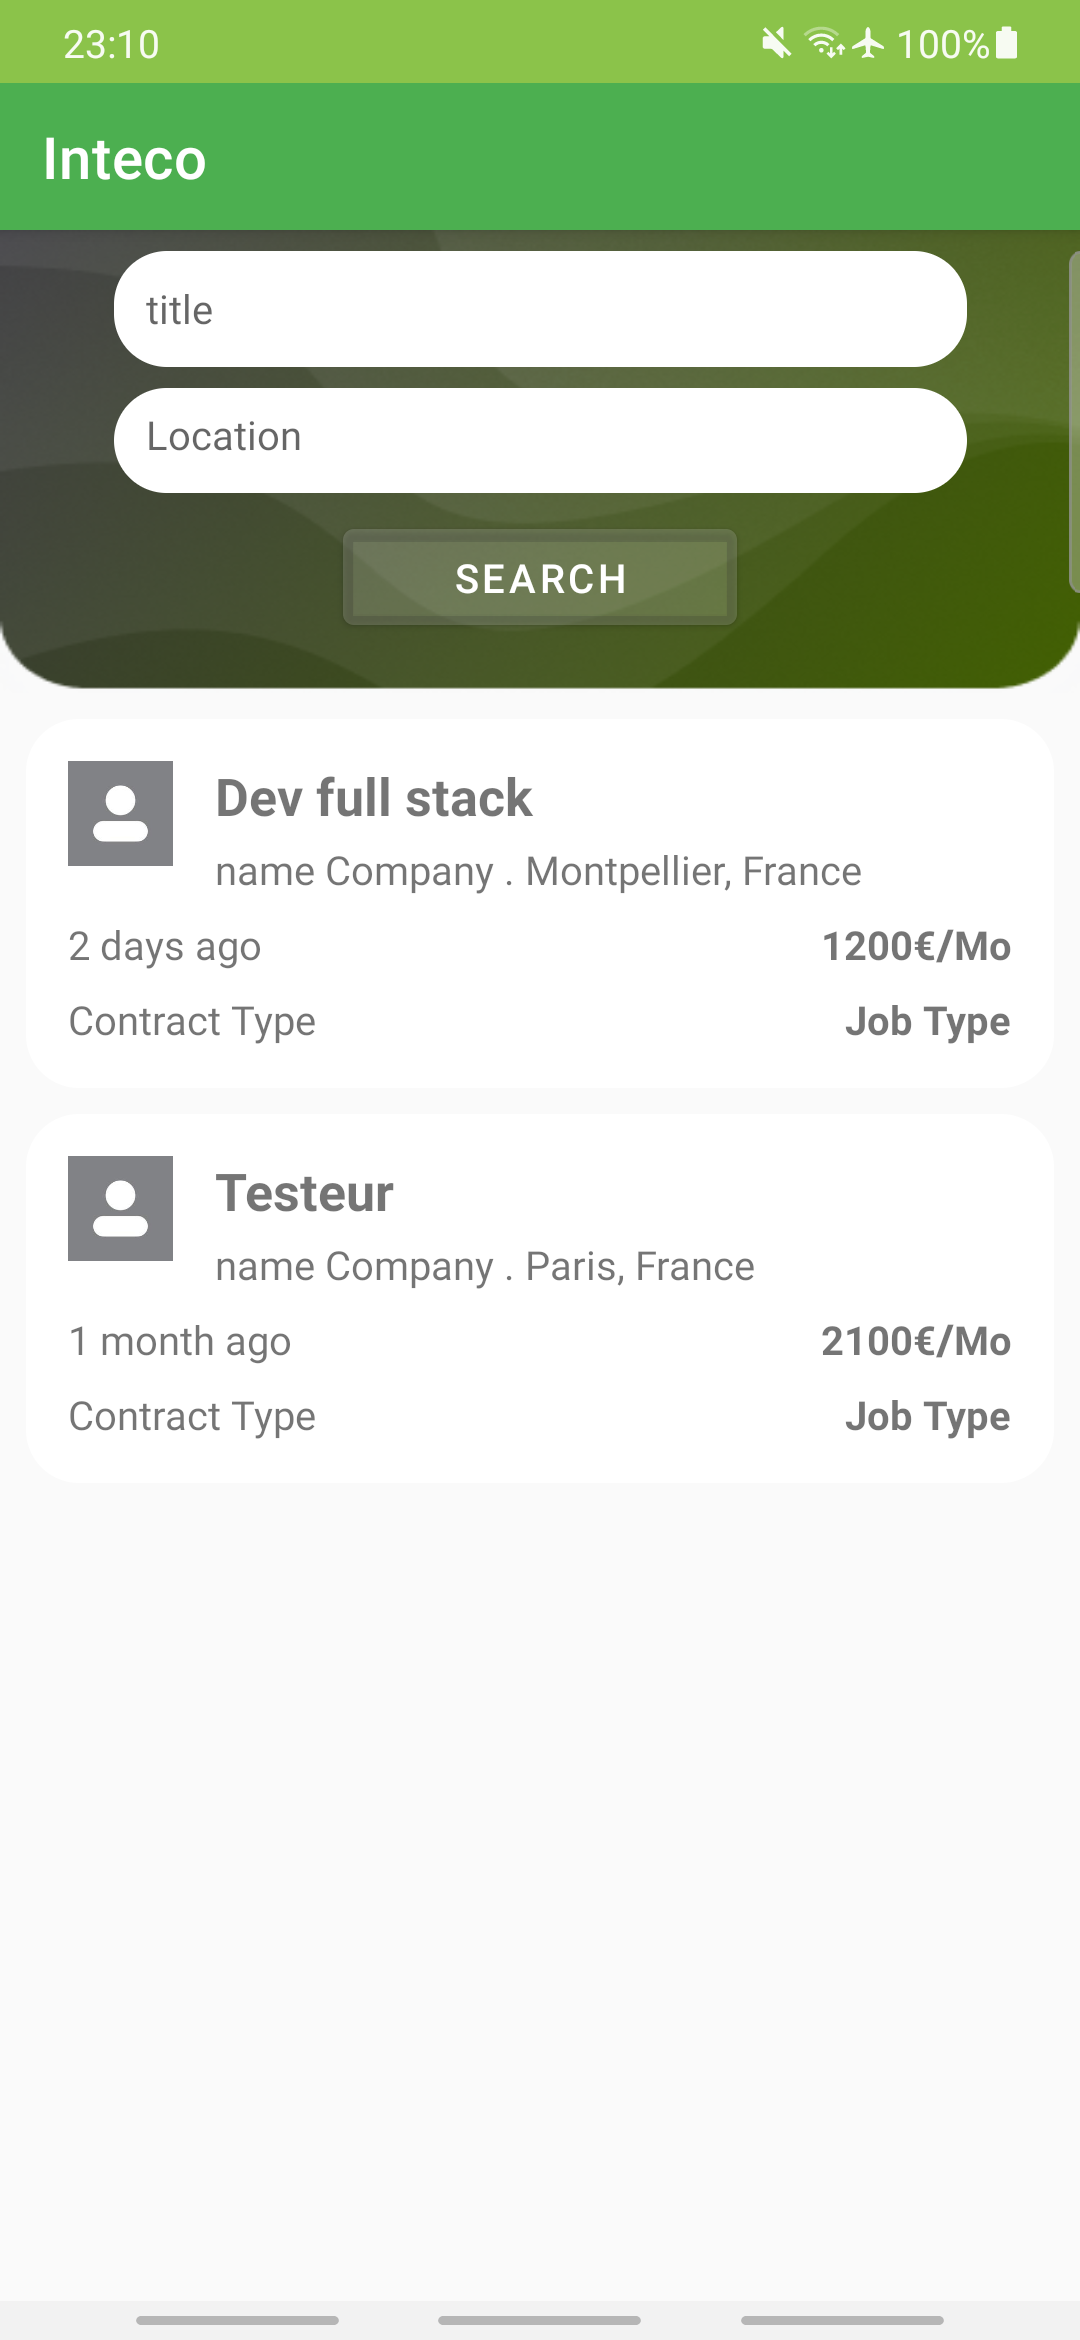
\includegraphics[width=.47\textwidth]{search/screenshotSearch}
        \noindent\includegraphics[width=.47\textwidth]{search/code}
    \end{multicols}
\end{document}